\documentclass[]{llncs}
\usepackage{times}
\usepackage{format}
\usepackage{macros}
\usepackage{macros_stm}
\usepackage{paper}
\usepackage{url}
\usepackage[colorlinks=true,linkcolor=blue,urlcolor=blue,citecolor=blue]{hyperref}
\begin{document}

\newboolean{showcomments}
\setboolean{showcomments}{false}
\ifthenelse{\boolean{showcomments}}
{ \newcommand{\mynote}[3]{
   \fbox{\bfseries\sffamily\scriptsize#1}
   {\small$\blacktriangleright$\textsf{\emph{\color{#3}{#2}}}$\blacktriangleleft$}}}
{ \newcommand{\mynote}[3]{}}
% One command per author:
\newcommand{\pf}[1]{\mynote{Pierre}{#1}{red}}
\newcommand{\hm}[1]{\mynote{Patrick}{#1}{pink}}
\newcommand{\vs}[1]{\mynote{Valerio}{#1}{blue}}
\newcommand{\ft}[1]{\mynote{Francois}{#1}{green}}

% tentative results 
% https://docs.google.com/spreadsheets/d/1jqpC7ehu48kJc96EYcEFRbjgV9wq8E9HbdZpwREfw7w/edit#gid=1043149494
% slides from euro-tm 2014
% https://docs.google.com/presentation/d/1AFntDVRBWmjOMjNzX90ZGo0cG4Jd7Pewas4CeemD5TQ/edit#slide=id.p

\title{Boosting Transactional Memory\\with Stricter Serializability%
  \thanks{
    This research is partly supported by the RainbowFS project of Agence Nationale de la Recherche, France, number ANR-16-CE25-0013-01a.
  }
}
%\titlerunning{} %only if title too long

\author{
  Pierre Sutra\inst{2}
  \and Patrick Marlier\inst{1}
  \and Valerio Schiavoni\inst{1} % \orcidID{0000-0003-1493-6603}
  \and Fran\c{c}ois Trahay\inst{2} % \orcidID{0000-0001-7329-1812}
}

\institute{
  University of Neuch\^atel, Switzerland
  % \email{\{patrick.marlier,valerio.schiavoni\}@unine.ch}
  \and
  T\'el\'ecom SudParis, France
  % \email{\{pierre.sutra,francois.trahay\}@telecom-sudparis.eu}
}


\maketitle

\noindent
\makebox[\linewidth]{\small Updated on August 2018}

\begin{abstract}
  Transactional memory (TM) guarantees that a sequence of operations encapsulated into a transaction is atomic.
  This simple yet powerful paradigm is a promising direction for writing concurrent applications.
  %
  Recent TM designs employ a time-based mechanism to leverage the performance advantage of invisible reads.
  With the advent of many-core architectures and non-uniform memory (NUMA) architectures, this technique is however hitting the synchronization wall of the cache coherency protocol.
  %
  To address this limitation, we propose a novel and flexible approach based on a new consistency criterion named stricter serializability ($\SPSER$).
  Workloads executed under $\SPSER$ are opaque when the object graph forms a tree and transactions traverse it top-down.  
  We present a matching algorithm that supports invisible reads, lazy snapshots, and that can trade synchronization for more parallelism.
  Several empirical results against a well-established TM design demonstrate the benefits of our solution.
  \keywords{Transactional memory \and NUMA \and stricter serializability}
\end{abstract}

\section{Introduction}
\labsection{introduction}

% why TM
The advent of chip level multiprocessing in commodity hardware has pushed applications to be more and more parallel in order to leverage the increase of computational power.
However, the art of concurrent programming is known to be a difficult task~\cite{Lee:2006:PT:1137232.1137289}, and new paradigms are required to help the programmer.
Among those paradigms, transactional memory (TM) is widely considered as a promising direction, in particular thanks to its simplicity~\cite{Dragojevic:2011:WSM:1924421.1924440}.

% the case for invisible optimistic reads and DAP
The engine that orchestrates concurrent transactions run by the application, i.e., the concurrency manager, is one of the core aspects of a STM implementation.
A large number of concurrency manager implementations exists, ranging from pessimistic lock-based implementations\vs{ref?} to completely optimistic ones\vs{ref?}, with~\cite{perelman2011smv} or without multi-version support\vs{ref?}.
Because application workloads exhibit in general a high degree of parallelism\vs{is this a known fact? for which applications? a ref that assess this statement would be good imho}, these designs tend to favor optimistic concurrency control.
In particular, a widely accepted approach consists in executing tentatively invisible read operations and validating them on the course of the transaction execution to enforce consistency.
Another property of interest is disjoint-access parallelism (DAP) \cite{}.
DAP ensures that concurrent transactions operating on disjoint part of the application do not contend in the concurrency manager.
This property is key to ensures that the system scales with the numbers of cores.

% why OPA
From a developper point of view, the interleaving of transactions must satisfy some form of correctness.
Strict serializability (SSER) is a consistency criteria commonly encountered in database litterature.
This criteria ensures committed transactions behave as if they were executed sequentially, in an order compatible with real-time.
Unfortunately, SSER does not say anything about transaction that abort.
For instance, the history $h_1$ below is allowed in SSER since transaction $T_1$ abort after reading inconsistent values for $x$ and $y$.
\begin{figure}[!h]
  \centering
  \fontsize{8}{11}\selectfont
  \begin{tikzpicture}[scale=0.77]
    \node at (10,.3) {$(h_1)$};
    
    \node at (0.2,1.8) {$T_1$};
    \node at (0.2,1) {$T_2$};
    
    \path[->] (0.5,1) edge (10,1);
    \path[->] (0.5,1.8) edge (10,1.8);
    
    \path[callA] (1.5,1.8) edge (2.5,1.8);
    \path[callA,->] (1.5,2) edge (1.5,1.8);
    \path[callA,->] (2.5,1.8) edge (2.5,2);
    \node at (1.5,2.2) {$r_1(x_0)$}; 
    \node at (2.5,2.2) {};

    \path[callA] (4,1.8) edge (5,1.8);
    \path[callA,->] (4,2) edge (4,1.8);
    \path[callA,->] (5,1.8) edge (5,2);
    \node at (4,2.2) {$r_1(y_2)$};
    \node at (5,2.2) {};

    \path[callA] (7,1.8) edge (8,1.8);
    \path[callA,->] (7,2) edge (7,1.8);
    \path[callA,->] (8,1.8) edge (8,2);
    \node at (7,2.2) {$\flagAbort$};
    \node at (8,2.2) {};

    \path[callB] (2.5,1) edge (3.5,1);
    \path[callB,->] (2.5,1.2) edge (2.5,1);
    \path[callB,->] (3.5,1) edge (3.5,1.2);
    \node at (2.5,1.4) {$w_2(x_2)$};
    \node at (3.5,1.4) {};

    \path[callB] (4.5,1) edge (5.5,1);
    \path[callB,->] (4.5,1.2) edge (4.5,1);
    \path[callB,->] (5.5,1) edge (5.5,1.2);
    \node at (4.5,1.4) {$w_2(y_2)$};
    \node at (5.5,1.4) {};

    \path[callB] (7,1) edge (8,1);
    \path[callB,->] (7,1.2) edge (7,1);
    \path[callB,->] (8,1) edge (8,1.2);
    \node at (7,1.4) {$\flagCommit$};
    \node at (8,1.4) {};
    
    \pgfresetboundingbox
    \clip[use as bounding box] (0,.7) rectangle (10,2);
  \end{tikzpicture}
\end{figure}

Opacity (OPA) was introduced to avoid the side-effects of so-called doom transactions, i.e., transactions which eventually abort (such as $T_1$ in history $h_1$).%
\footnote{  
  Allowing $T_1$ to return both $x_0$ and $y_2$ may have dire consequences in a non-managed environement.
  For instance \cite{opa}, transaction $T_1$ may compute a division by $0$, leading the program to crash.
}
In addition to SSER, OPA requires that aborted transactions observe a prefix of the committed transactions.
This is the usual consistency criteria for TM.

% the cost of achieving OPA
Achieving OPA is known to be expensive, even for weak progess properties on the transactions \cite{}.
In particular, ensuring that a transaction always observes a consistent snapshot when read are invisible require to either validate the read set after each read operation, or to rely on a global clock.
The former approach results in a quadratic-time validation complexity.
The latter approach is expensive in multi-core/multi-processors architecture, due to a synchronization wall.

% our contributions
In this paper, we address these shortcomings with a new consistency criteria, named stricter serializability (S+SER).
This criteria extends strict serializability while avoiding the inconsistency depicted in history $h_1$.
We present a matching TM algorithm that ensures DAP, invisible reads, and permits transactions to commit as long as they do do contend with conflicting transactions.
We then validate our design by means of a full implementation and several experiments.
Our result shows that when the workloads is strongly parallelism, our algorithm offers performance close to the optimum.

\textbf{Outline.}
The outline of this paper is as follows.
\refsection{criteria} introduces S+SER.
The algorithm and a formal proof of its correctnesss are presented in ~\refsection{stm}
\refsection{evaluation} presents our extensive evaluation against several benchmarks.
We survey related work in \refsection{relatedwork}.
\refsection{conclusion} closes this paper.

\section{A new consistency criterion}
\labsection{criterion}

This section is organized in four parts.
The first part (\refsection{criterion:model}) presents the elements of our system model.
Further, the notions of contention and binding (\refsection{criterion:bindings}) are introduced.
These notion are used to define stricter serializability (\refsection{criterion:spser}) and to study its applicability (\refsection{criterion:applicability}).

\subsection{System model}
\labsection{criterion:model}

Transactional memory (TM) is a recent paradigm that allows multiple processes to access concurrently a shared memory region.
Each process manipulates \emph{objects} in the shared memory with the help of transactions.
% object -> data item.

When a process starts a new transaction, it calls operation \stmBeginFunction.
Then, the process executes a sequence of \stmReadFunction and \stmWriteFunction operations on the shared objects according to some internal logic.
Operation \stmRead{x} takes as input an object $x$ and returns either a value in the domain of $x$ or a flag $\flagAbort$ to indicate that the transition aborts.
A write \stmWrite{x,v} changes $x$ to the value $v$ in the domain of $x$.
This operation does not return any value and it may also abort.
Without lack of generality, we consider that a transaction reads or writes to a given shared object at most once.
At the end of the transaction execution, the process calls \stmTryCommitFunction to complete the transaction.
This calls returns either $\flagCommit$, to indicate that the transaction was successful, or $\flagAbort$ if the transaction fails.
When the transaction aborts or commits, it takes no further step.

A \emph{history} is a sequence of invocations and responses of TM operations by one or more processes.
As illustrated with history $h_2$ below, a history is commonly depicted as parallel timelines, one per process, and each timeline consists of the sequence of transactions executed at that process.

\begin{figure}[!h]
  \centering
  \fontsize{8}{11}\selectfont
  \begin{tikzpicture}[scale=0.77]
    \node at (10,.3) {$(h_2)$};

    \node at (0.2,2.6) {$T_1$};
    \node at (0.2,1.8) {$T_2$};
    \node at (0.2,1) {$T_3$};

    \path[->] (0.5,2.6) edge (10,2.6);
    \path[->] (0.5,1.8) edge (10,1.8);
    \path[->] (0.5,1) edge (10,1);
    
    \path[callA] (2,2.6) edge (3,2.6);
    \path[callA,->] (2,2.8) edge (2,2.6);
    \path[callA,->] (3,2.6) edge (3,2.8);
    \node at (2,3) {$w_1(x_1)$}; 
    \node at (3,3) {};

    \path[callA] (4,2.6) edge (5,2.6);
    \path[callA,->] (4,2.8) edge (4,2.6);
    \path[callA,->] (5,2.6) edge (5,2.8);
    \node at (4,3) {$\flagCommit$};
    \node at (5,3) {};

    \path[callB] (1.5,1.8) edge (2.5,1.8);
    \path[callB,->] (1.5,2) edge (1.5,1.8);
    \path[callB,->] (2.5,1.8) edge (2.5,2);
    \node at (1.5,2.2) {$w_2(x_2)$}; 
    \node at (2.5,2.2) {};

    \path[callB] (3.5,1.8) edge (4.5,1.8);
    \path[callB,->] (3.5,2) edge (3.5,1.8);
    \path[callB,->] (4.5,1.8) edge (4.5,2);
    \node at (3.5,2.2) {$\flagCommit$};
    \node at (4.5,2.2) {};

    \path[callC] (5,1) edge (6,1);
    \path[callC,->] (5,1.2) edge (5,1);
    \path[callC,->] (6,1) edge (6,1.2);
    \node at (5,1.4) {$r_3(x_1)$};
    \node at (6,1.4) {};

    \path[callC] (7,1) edge (8,1);
    \path[callC,->] (7,1.2) edge (7,1);
    \path[callC,->] (8,1) edge (8,1.2);
    \node at (7,1.4) {$\flagCommit$};
    \node at (8,1.4) {};
    
    \pgfresetboundingbox
    \clip[use as bounding box] (0,.7) rectangle (10,2.8);
  \end{tikzpicture}
\end{figure}


In history $h_2$, process $p$, $q$ and $r$ execute respectively transactions ${\color{blue}{T_1}}=w(x)$, ${\color{red}{T_2}}=w(x)$ then ${\color{Purple}{T_4}}=r(y);r(x)$, and ${\color{OliveGreen}{T_3}}=r(x);w(y)$.
In this history, transactions $T_1$, $T_2$ and $T_3$ all \emph{complete}, whereas transaction $T_4$ is \emph{live}.
For clarity, calls to $\stmBeginFunction$ are omitted in such diagrams and every complete transaction which is not explicitly aborted commits immediately after its last operation.

We note $\committed{h}$ the set of transactions that commit during history $h$.
In the case of history $h_2$, we have $\committed{h_2}=\{T_1,T_2,T_3\}$.

Over the course of its execution, a transaction $T_i$ reads and writes one or more versions of the shared objects.
The set of versions read by the transaction forms its \emph{read set} (denoted $\readSetOf{T_i}$).
The versions written during the execution define the \emph{write set} ($\writeSetOf{T_i}$).

A \emph{version} is the state of a shared object as produced by a write operation.
When a transaction $T_i$ writes to some object $x$, an operation denoted $w_i(x_i)$, it creates the version $x_i$ of $x$.
Versions allow to uniquely identify the state of an object as observed by a read operation, \emph{e.g.}, $r_3(x_1)$ in $h_2$.
We shall say that version $x_i$ is committed when $T_i$ commits in the history.

A history induces a real-time order between transactions (denoted $\hb_h$).
% TODO omit subscripts.
The order $T_i \hb_h T_j$ holds when $T_i$ completes in $h$ before $T_j$ begins.
For instance in history $h_2$, transaction $T_1$ precedes transaction $T_3$.
When transactions $T_i$ and $T_j$ are not related with real-time, they are \emph{concurrent} (denoted $T_i \cc_h T_j$).

History $h$ is \emph{complete} when it contains no live transaction.
Histories $h$ and $h'$ are \emph{equivalent} ($h \equiv h'$) when they contain the same events.
A history $h$ is \emph{sequential} when no two transactions are concurrent in $h$.
A sequential history $h$ is \emph{legal} when for every read $r_i(x_j)$ in $h$, $T_j$ is the last committed transaction before $T_i$ that writes to $x$ in $h$.

For some history $h$, a version order on object $x$ for $h$ is a total order over all the versions $x_i$ such that $T_i$ commits in $h$.
% TODO define everything without this (non-standard) assumption 
By extension, a version order for $h$ (written $\ll_h$) is a union of version orders, one per object.
As an example, in history $h_2$ above, we may consider the version order $(x_2 \ll_{h_2} x_1)$.

Consider a history $h$, some version order $\ll_h$ and two distinct transactions $T_i$ and $T_j$ in $h$.
Following \cite{Adya99}, we shall say that:
% FIXME in \cite{}, ``direct'' relations are only considered.
\begin{compactitem}
\item $T_j$ \emph{read-depend} on $T_i$ when $r_j(x_i)$ occurs in $h$ ($T_i \wrdep T_j$);
\item $T_j$ \emph{write-depends} on $T_i$ when $x_i \ll_h x_j$ is true ($T_i \wwdep T_j$); and
\item $T_j$ \emph{anti-depends} on $T_i$ when $r_i(x_k) \in h \land x_k \ll_h x_j$ holds ($T_i \adep T_j$).
\end{compactitem}
To illustrate the above definitions, consider again history $h_2$, with $x_2 \ll_h x_1$.
In this history, transaction $T_3$ read-depends on $T_1$ and $T_1$ write-depends on $T_2$.
Moreover, if transaction $T_4$ reads $x_2$, then $T_1$ anti-depends on $T_4$.

Consider that $T_j$ anti-depends on $T_i$ because it updates some object $x$ and $T_i$ reads a prior version.
This anti-dependency is a \emph{reverse-commit anti-dependency} (for short, RC-anti-dependency) \cite{hans16} when $T_j$ invokes $\stmTryCommitFunction$ before $T_i$ in $h$, and $T_i$ writes to some object $y \neq x$.
%
\footnote{
  By not requiring that $T_j$ reads $x$ before updating it, this definition slightly generalizes the notion of RC-anti-dependency as introduced in \cite{hans16}.
}

In what follows, we assume that every history is complete and that read operation always returns a committed version.
% r_i(x_j) \in h \implies \neg (r_i(x_j) \hb_h \stmTryCommitFunction_j)
These simplifying assumptions are motivated by the fact that TM designs favor wait-free operations and buffer updates until commit \cite{bookTM}.
% TODO remove these assumptions

\subsection{Contention and bindings}
\labsection{criterion:bindings}

Internally, a transactional memory is built upon a set of \emph{base objects}, such as locks and registers.
When two transactions are concurrent, their steps on these base objects interleave.
If two transactions access distinct objects and the TM is disjoint-access parallel, no contention occurs.
However, in the case they access the same base object, they may slow down each other.

A transactional read is \emph{invisible} when it does not change the state of the base objects implementing it.
With invisible reads, read contention is basically free.
From a performance point of view, this property is consequently appealing, since workloads exhibit a large ratio of read operations \cite{stampBenchmark}.

When two transactions are concurrently writing to the same object, it is possible to detect the contention and abort preemptively one of them.
On the other hand, when a read-write conflict happens, a \emph{race condition} occurs between the reader and the writer.
If the read operation takes place after the write, the reader is bound to use the version produced by the writer.
% when x_j is visible, all its dependencies are also visible.
% thus, if x_j is visible before T_i begins its execution, no dependency can be missed.
% this only happens when the two transactions are concurrent.

\begin{definition}[Binding]
  During a history $h$, when $T_i$ and $T_j$ are concurrent and $r_i(x_j)$ occurs in $h$, we say that $T_i$ is bound to $T_j$ on $x$.
\end{definition}

When transaction $T_i$ is bound to $T_j$, to preserve the consistency of its read set, $T_i$ must observe the dependencies of $T_j$.
This is for instance the case of transaction $T_4$ in history $h_2$, where this transaction is bound to $T_3$ on $y$.
As a consequence, $T_4$ must return $x_1$ as the result of its read on $x$, or its read set will be not be consistent.

\begin{definition}[Dependency]
  Consider some version order $\ll_h$ for $h$.
  We say that $T_j$ \emph{depends} on $T_i$ ($T_i \rdepends T_j$)  when $T_j$ read-depends or write-depends on $T_i$, directly or by transitivity.
  In other words, $\rdepends$ equals $\closureOf{((\wrdep) \union (\wwdep))}$, where $\closureOf{R}$ denotes the transitive closure of the binary relation $R$,
  For readability, we also define $T_j \depends T_i$ as $T_i \rdepends T_j$.
  % TODO to fix.
\end{definition}

Tracking dependencies is difficult for the TM since it requires to re-validate the read set after each read, rely on a global clock, or use large amount of metadata.
We observe that this computation is simplified when each version read before the binding is either a dependency of the version newly read, or was installed after it.
In which case, we will say that the binding is fair.

\begin{definition}[Fair binding]
  Consider that in some history $h$ a transaction $T_i$ is bound to a transaction $T_j$ on some object $x$.
  This binding is \emph{fair} when, for every version $y_k$ read by $T_i$ before $x_j$ in $h$, $T_j \depends_h T_k$ holds, or $T_k$ invokes $\stmTryCommitFunction$ after $T_j$.
\end{definition}

Going back to history $h_2$, the binding of $T_4$ to $T_3$ on $y$ is fair.
Indeed, this transaction did not read any data item before accessing the version of $y$ written by $T_3$.

When the binding is fair, the reader can leverage the metadata left by the writer to check prior versions it has read and ensure that its read set is consistent.
In the next section, we formalize this idea with the notion of stricter serializability.

\subsection{Stricter serializability}
\labsection{criterion:spser}

In what follows, we introduce and describe in detail \SPSER, the stricter serializability consistency criterion that we build upon in the remainder of this paper.
As strict serializability, \SPSER requires that committed transactions form a sequential history which preserves the real-time order.
In addition, it prohibits transactions to view inconsistencies unless one of their bindings is unfair.

For a history $h$ and some version order $\ll_h$, $<_h$ captures all the constrains on the ordering of transactions in $h$.
In other words, $<_h$ equals $((\wrdep) \union (\wwdep) \union (\adep) \union (\hb_h))$.
We note $<_{\committed{h}}$ the restriction of $<_{h}$ to the transactions committed in $h$.

\begin{definition}[Strict serializability \cite{Adya99}]
  The real-time serialization graph of history $h$ induced by $\ll_h$, written $\RSG(h,\ll_h)$, is defined as $(\committed{h},<_{\committed{h}})$.  
  History $h$ is \emph{strictly serializable} ($h \in \SSER)$ when $\RSG(h,\ll_h)$ is acyclic for a version order $\ll_h$.
\end{definition}

If history $h$ is strictly serializable, linearizing the transactions committed in $h$ following $<_{\committed{h}}$ leads to a legal history.
% TODO \cite{} ?
However, as pointed out in the introduction, \SSER does not constraint the behavior of aborted transactions which may behave arbitrary.
Opacity ($\OPA$) extends strict serializability to avoid such situations.

\begin{definition}[Opacity \cite{guerraoui2008correctness}]
  A history $h$ is opaque ($h \in \OPA$) when there exists a sequential and legal history $\lambda$ equivalent to $h$ that preserves the real-time order in $h$ (that is, $\hb_{\lambda} \subseteq \hb_{h}$).
\end{definition}

In this paper, we are interested in bridging the gap between strict serializability and opacity.
To this end, we need first to introduce the notion of strictly consistent snapshot. 

\begin{definition}[Strictly consistent snapshot]
  Consider some history $h$ and a version order $\ll_h$.
  A transaction $T_i$ observes a \emph{strictly consistent snapshot} for $\ll_h$ when the transitive closure of $<_h$ starting from $\{T_i\}$ is acyclic.
  % TODO for every read $r_i(x_{j \neq i})$ in $h$, $T_j$ commits in $h$, and
  %      writes also need to take place before, otherwise the prefix is invalid (theoretically this ofc is not a problem).
\end{definition}

Our \SPSER criterion requires that after each read operation, the transactions sees a strictly consistent snapshot or one of its bindings is unfair.

\begin{definition}[Stricter serializability]
  \labdef{spser}
  A history $h$ is stricter serializable ($h \in \SPSER$) when for some version order $\ll_h$,
  \begin{inparaenum}
  \item $\RSG(h,\ll_h)$ is acyclic, and
  \item for every transaction $T_i$ that aborts in $h$, either $T_i$ observes a strictly consistent snapshot for $\ll_h$, or one of its binding is unfair.
  \end{inparaenum}
\end{definition}

A strictly serializable history becomes opaque when aborted transactions read strictly consistent snapshots.
(We provide a rigorous proof for this claim in \refappendix{from}.)
As a consequence of the above definition, a stricter serializable history during which all the aborted transactions exhibit fair bindings is opaque.
The next section gives a class of applications for which this characterization is true.
In other words, we present a robustness criterion~\cite{CeroneG16} against $\SPSER$.

\subsection{Applicability}
\labsection{criterion:applicability}

In what follows, we detail the model of application we are interested with.
Then, we present our robustness criterion and prove that it applies to $\SPSER$.

\subsubsection{Model of application}
\labsection{criterion:app}

The state of an object commonly includes \emph{references} to one or more other objects in the shared memory.
These references between objects form the \emph{object graph} of an application.

When performing a computation, a process traverses the object graph.
To this end, the process knows initially an immutable root object in the graph.
Starting from this root, the process executes a traversal by using the references stored in each object.

For some transaction $T_i$, a \emph{path} is the sequence of versions $\pi_i$ read by $T_i$.
It should satisfy that 
\begin{inparaenum}
\item the first object in $\pi_i$ corresponds to the immutable root of the object graph, and
\item for all $x_j \in \pi_i$, some $y_k <_{\pi} x_j$ includes a reference to $x_j$.
\end{inparaenum}

A path $\pi_i$ is \emph{simple} when for all $k \in [1,\cardinalOf{\pi_i}]$, $\pi_i[k]$ includes a reference to $\pi_i[k+1]$.
When a path is simple, for some object $x$, $\pi_{i,x}$ and $\hat{\pi}_{i,x}$ are respectively the paths from the root to $x$ before and after transaction $T_i$.
Hereafter, when writing $\pi_{i,x}$, and $\hat{\pi}_{i,x}$, we implicitly assume that such a path exists.

\subsubsection{Robustness}
\labsection{criterion:robustness}

To define our robustness criterion, we focus specifically on $\SPSER$ implementations that allow invisible reads.
As pointed out earlier, this restriction is motivated by performance as most workloads are read-intensive.
In this context, the result of Hans et al. \cite{hans16} tells us that it is not possible to jointly achieve
\begin{inparaenum}
\item $\SSER$,
\item read invisibility,
\item minimal progressiveness, and
\item accept RC-anti-dependencies.
\end{inparaenum}
% TODO. this is an approximation of the real result of Hans et al. 
As a consequence, we remove histories that exhibit such a pattern from our analysis; hereafter, we shall note $\RCAD$ these histories.

Let us consider property $\mathcal{P}$ on a TM application as defined below.
Hereafter, we name $\mathcal{T}$ some set of transactions for which property $\mathcal{P}$ holds and let $H_{\mathcal{T}}$ refer to the histories built upon transactions in $\mathcal{T}$.
\begin{itemize}
\item[($\mathcal{P}$)]
  The object graph forms initially a tree and every transaction maintains this invariant.
  Moreover, every transaction in the application follows a simple path.
\end{itemize}
We wish to establish the following result:

\begin{proposition}
  \labprop{criterion:2}
  $(\SPSER \inter H_{\mathcal{T}} \setminus \RCAD) \subset \OPA$.
\end{proposition}

To state this result, we note $h$ some history  in $(\SPSER \inter H_{\mathcal{T}} \setminus \RCAD)$.
Since $h$ is serializable, there exists some sequential history $\lambda$ equivalent to $\committed{h}$.

\begin{lemma}
  \lablem{criterion:1}
  If $T_i \hb_{\lambda} T_j$ holds and $T_j$ reads $x$ in $\lambda$, then for every $y_k \in \hat{\pi}_{i,x}$, $T_j \depends_h T_k$ is true.
  % TODO. path wrt. \lambda
\end{lemma}

\begin{proof}

  Since $T_j$ reads $x$, $\pi_{j,x} \subseteq \readSetOf{T_j}$.
  Then, for some $y_k \in \hat{\pi}_{i,x}$, two cases are possible:
  \begin{itemize}
  \item ($\exists T_l \in \lambda : y_l  \in \pi_{j,x}$)
    The claim trivially holds if $l = k$.
    If now $l \neq k$, $T_i \hb_{\lambda} T_j$ implies that $T_k \hb_{\lambda} T_l$.
    Hence, $y_k \ll_{h} y_l$ is true leading to $T_j \depends_h T_k$.
  \item (Otherwise.)
    Let $T_l \hb_{\lambda} T_j$ be the transaction that deletes $y$ from the object graph.
    Without lack of generality assume this was still version $y_k$.
    Because $\pi_{j,x}$ is defined and property $\mathcal{P}$ holds, $\hat{\pi}_{l,x}$ is defined.
    By property $\mathcal{P}$, there exist $z_{?}$ and $t_{\versionAny}$ such that
    $\pi_{l,x} = \ldots z_{?} \ldots y_{k} \ldots t_{\versionAny} \ldots$
    and $\hat{\pi}_{l,x} = \ldots z_{l}t_{\versionAny} \ldots$, and transaction $T_l$ reads version $y_{k}$.
    Now, if $z_l$ is in $\pi_{i,x}$, $T_j \depends_h T_k$ holds.
    In the converse case, we repeat the above reasoning for $z_l$.
  \end{itemize}     
    
\end{proof}

\begin{corollary}
  \labcor{criterion:1}
  The relation $T_i \depends_h T_k$ holds for every version $y_k$ in ($\pi_{i,x} \union \hat{\pi}_{i,x}$).
\end{corollary}

\begin{lemma}
  \lablem{criterion:2}
  If transaction $T_i$ aborts in $h$ then all its bindings are fair.
\end{lemma}

\begin{proof}

  (By induction.)
  Define $x$ and $T_j$ such that $T_i$ is bound to $T_j$ on $x$ and assume that all the prior bindings (if any) of $T_i$ are fair.
  It follows that transaction $T_i$ observes a strictly consistent snapshot in $h$ before $r_i(x_j)$.
  Hence, there exists a committed transaction $T_k$ such that $\pi_{i,x}$ is the path to $x$ after transaction $T_k$ in $\lambda$ (i.e., $\hat{\pi}_{k,x}= \pi_{i,x}$).
  % FIXME $T_i$ observes a strictly consistent snapshot in $h'$ = h \setminus {the read operation after r_i(x_j) }.
  % FIXME prove this.
  Let us prove that $r_i(x_j)$ is fair.
  Depending on the relative positions of $T_j$ and $T_k$ in $\lambda$, there are two cases to consider.
  \begin{itemize}
  \item $(T_k \hb_{\lambda} T_j)$.
    This case is a direct application of \reflem{criterion:1}.
  \item $(T_j = T_k) \lor (T_j \hb_{\lambda} T_k)$.
    If $\pi_{i,x} = \hat{\pi}_{j,x}$ holds, then \refcor{criterion:1} tells us that $r_i(x_j)$ is fair.
    %
    Otherwise, there exists some transaction $T_l$ such that $T_j \hb_{\lambda} T_l \hb_{\lambda} T_k$ and $T_l$ modifies $\hat{\pi}_{j,x}$.
    Without lack of generality, assume $T_l$ to be the first such transaction.
    If $T_l$ invokes $\stmTryCommitFunction$ after transaction $T_j$, then the binding is fair.
    In the converse case, $T_l$ does not observe any modification made by $T_j$.
    % FIXME strictly consistent snapshot -> committed values only.
    Hence, $T_l$ modifies the path $\pi_{j,x}$.
    In order to maintain invariant $\mathcal{P}$, transaction $T_l$ must update some object $z$ read in $\pi_{j,x}$.
    Because $T_l$ invokes $\stmTryCommitFunction$ before $T_j$, yet $T_j \hb_{\lambda} T_l$, the two transactions are concurrent in $h$.
    Hence, history $h$ exhibits an RC-anti-dependency between $T_j$ and $T_l$ on object $z$.
    Contradiction.
  \end{itemize}
\end{proof}

\section{Algorithm}
\labsection{stm}

In this section, we depict a locality-aware software transactional memory.
The pseudo-code of our construction is presented in \refalg{stm}.
This algorithm follows the general design of the lazy snapshot algorithm (LSA) of \citet{FelberFMR10}, replacing the central clock with a more flexible mechanism.

In what follows, we give an overview of the algorithm, present its internals then justify some design choices.
A correctness proofs follows.

\subsection{Overview}
\labsection{stm:overview}

\refalg{stm} depicts the pseudo-code of our implementation of the STM interface at some process $p$.
Our design follows a deferred update schema that consists in two steps.
A transaction first executes optimistically, buffering its updates.
Then at commit time the transaction is certified and, provided it commits, its updates are applied to the shared memory.

During the execution of a transaction, process $p$ checks that the registers accessed so far did not change.
Similarly to LSA, this check is lazily executed.
\refalg{stm} executes it only when a register appears to have been recently updated, or when transaction terminates.

\subsection{Tracking Time}
\labsection{stm:time}

%% define consistent clock as any mechanism from $H$ to (\tickSet,<)
%% satisfying for any two e, e' in $H$, $\hb e' \implies \Theta(e) < \Theta(e')$.

\refalg{stm} tracks time to compute how concurrent transactions interleave during an execution.
To this end, the algorithm makes use of logical clocks.
We model the interface of a \emph{logical clock} with two operations: $\cread$ returns a value in $\naturalSet$, and $\cadv(v \in \naturalSet)$ updates the clock with value $v$.
The sequential specification of a logical clock guarantees a single property, that the time flows forward:
\begin{inparaenum}
\item[\emph{(Time monoticity)}]
  A read operation always returns at least the greatest value to which the clock advanced so far.
  Formally, for every history $h$, $(\responseAny{\cread}{v} \in h) \implies (v \geq \max{(\{u : \cadv(u) \hb_h \cread \} \union \{0\})})$.
\end{inparaenum}

\refalg{stm} associates logical clocks with both processes and transactions.
To retrieve the clock associated with some object $i$, our algorithm uses function $\clockOf{i}$.
Notice that in the pseudo-code, when it is clear from the context, 
we write $\clockOf{i}$ as a shorthand for $\clockOf{i}.\mathit{read}()$.

The clock associated with a transaction is always local (\refline{stm:var:1}).
In the case of a process, it might be shared or not (\refline{stm:var:2}).
The flexibility of our design comes from this locality choice for \clockOf{p}.
When the clock is shared, it is linearizable.
To implement an (obstruction-free) linearizable clock we proceeds as follows.
\begin{construction}
  Let $x$ be a shared register initialized to $0$.
  When $\cread$ is called, we return the value stored in $x$.
  Upon executing $\cadv(v)$, we fetch the value stored in $x$, say $u$.
  If $v > u$ holds, we execute a compare-and-swap to replace $u$ with $v$; 
  otherwise the operation returns.
  If the compare-and-swap fails, the previous steps are retried.
\end{construction}

\section{Algorithm}
\labsection{stm}

In this section, we depict a locality-aware software transactional memory.
The pseudo-code of our construction is presented in \refalg{stm}.
This algorithm follows the general design of the lazy snapshot algorithm (LSA) of \citet{FelberFMR10}, replacing the central clock with a more flexible mechanism.

In what follows, we give an overview of the algorithm, present its internals then justify some design choices.
A correctness proofs follows.

\subsection{Overview}
\labsection{stm:overview}

\refalg{stm} depicts the pseudo-code of our implementation of the STM interface at some process $p$.
Our design follows a deferred update schema that consists in two steps.
A transaction first executes optimistically, buffering its updates.
Then at commit time the transaction is certified and, provided it commits, its updates are applied to the shared memory.

During the execution of a transaction, process $p$ checks that the registers accessed so far did not change.
Similarly to LSA, this check is lazily executed.
\refalg{stm} executes it only when a register appears to have been recently updated, or when transaction terminates.

\subsection{Tracking Time}
\labsection{stm:time}

%% define consistent clock as any mechanism from $H$ to (\tickSet,<)
%% satisfying for any two e, e' in $H$, $\hb e' \implies \Theta(e) < \Theta(e')$.

\refalg{stm} tracks time to compute how concurrent transactions interleave during an execution.
To this end, the algorithm makes use of logical clocks.
We model the interface of a \emph{logical clock} with two operations: $\cread$ returns a value in $\naturalSet$, and $\cadv(v \in \naturalSet)$ updates the clock with value $v$.
The sequential specification of a logical clock guarantees a single property, that the time flows forward:
\begin{inparaenum}
\item[\emph{(Time monoticity)}]
  A read operation always returns at least the greatest value to which the clock advanced so far.
  Formally, for every history $h$, $(\responseAny{\cread}{v} \in h) \implies (v \geq \max{(\{u : \cadv(u) \hb_h \cread \} \union \{0\})})$.
\end{inparaenum}

\refalg{stm} associates logical clocks with both processes and transactions.
To retrieve the clock associated with some object $i$, our algorithm uses function $\clockOf{i}$.
Notice that in the pseudo-code, when it is clear from the context, 
we write $\clockOf{i}$ as a shorthand for $\clockOf{i}.\mathit{read}()$.

The clock associated with a transaction is always local (\refline{stm:var:1}).
In the case of a process, it might be shared or not (\refline{stm:var:2}).
The flexibility of our design comes from this locality choice for \clockOf{p}.
When the clock is shared, it is linearizable.
To implement an (obstruction-free) linearizable clock we proceeds as follows.
\begin{construction}
  Let $x$ be a shared register initialized to $0$.
  When $\cread$ is called, we return the value stored in $x$.
  Upon executing $\cadv(v)$, we fetch the value stored in $x$, say $u$.
  If $v > u$ holds, we execute a compare-and-swap to replace $u$ with $v$; 
  otherwise the operation returns.
  If the compare-and-swap fails, the previous steps are retried.
\end{construction}

\section{Algorithm}
\labsection{stm}

In this section, we depict a locality-aware software transactional memory.
The pseudo-code of our construction is presented in \refalg{stm}.
This algorithm follows the general design of the lazy snapshot algorithm (LSA) of \citet{FelberFMR10}, replacing the central clock with a more flexible mechanism.

In what follows, we give an overview of the algorithm, present its internals then justify some design choices.
A correctness proofs follows.

\subsection{Overview}
\labsection{stm:overview}

\refalg{stm} depicts the pseudo-code of our implementation of the STM interface at some process $p$.
Our design follows a deferred update schema that consists in two steps.
A transaction first executes optimistically, buffering its updates.
Then at commit time the transaction is certified and, provided it commits, its updates are applied to the shared memory.

During the execution of a transaction, process $p$ checks that the registers accessed so far did not change.
Similarly to LSA, this check is lazily executed.
\refalg{stm} executes it only when a register appears to have been recently updated, or when transaction terminates.

\subsection{Tracking Time}
\labsection{stm:time}

%% define consistent clock as any mechanism from $H$ to (\tickSet,<)
%% satisfying for any two e, e' in $H$, $\hb e' \implies \Theta(e) < \Theta(e')$.

\refalg{stm} tracks time to compute how concurrent transactions interleave during an execution.
To this end, the algorithm makes use of logical clocks.
We model the interface of a \emph{logical clock} with two operations: $\cread$ returns a value in $\naturalSet$, and $\cadv(v \in \naturalSet)$ updates the clock with value $v$.
The sequential specification of a logical clock guarantees a single property, that the time flows forward:
\begin{inparaenum}
\item[\emph{(Time monoticity)}]
  A read operation always returns at least the greatest value to which the clock advanced so far.
  Formally, for every history $h$, $(\responseAny{\cread}{v} \in h) \implies (v \geq \max{(\{u : \cadv(u) \hb_h \cread \} \union \{0\})})$.
\end{inparaenum}

\refalg{stm} associates logical clocks with both processes and transactions.
To retrieve the clock associated with some object $i$, our algorithm uses function $\clockOf{i}$.
Notice that in the pseudo-code, when it is clear from the context, 
we write $\clockOf{i}$ as a shorthand for $\clockOf{i}.\mathit{read}()$.

The clock associated with a transaction is always local (\refline{stm:var:1}).
In the case of a process, it might be shared or not (\refline{stm:var:2}).
The flexibility of our design comes from this locality choice for \clockOf{p}.
When the clock is shared, it is linearizable.
To implement an (obstruction-free) linearizable clock we proceeds as follows.
\begin{construction}
  Let $x$ be a shared register initialized to $0$.
  When $\cread$ is called, we return the value stored in $x$.
  Upon executing $\cadv(v)$, we fetch the value stored in $x$, say $u$.
  If $v > u$ holds, we execute a compare-and-swap to replace $u$ with $v$; 
  otherwise the operation returns.
  If the compare-and-swap fails, the previous steps are retried.
\end{construction}

\input{algorithms/stm.tex}

\subsection{Details}
\labsection{stm:detail}

In \refalg{stm}, each register $x$ has a \emph{location} in the shared memory, denoted $\locationOf{x}$.
This location stores a pair $(t,d)$, where $t \in \naturalSet$ is a \emph{timestamp}, and $d$ is the actual content of $x$ as seen by transactions.
We name a pair $(t,d)$ a \emph{version} of the register $x$.
Since the location of register $x$ is unique, a single version of register $x$ may exist at a time in the memory.
As usual, we asume some transaction $\transInit$ that intializes for every register $x$ the location $\locationOf{x}$ to $(0,\bot)$.
Furthermore, we consider that each register $x$ is atomic.

\refalg{stm} associates each register with a lock.
To manipulate the lock-related functions of register $x$, 
a process $p$ employs appropriately the functions $\lock{x}$, $\isLocked{x}$ and $\unlock{x}$.

For every transaction $T$ submitted to the system, \refalg{stm} maintains three local data structures:
\begin{inparaenum}[]
\item $\clockOf{T}$ is the logical clock of transaction $T$,
\item $\readSetOf{T}$ is a map that contains its \emph{read set}, and 
\item $\writeSetOf{T}$ is another map that stores the \emph{write set} of $T$.
\end{inparaenum}
\refalg{stm} updates incrementally $\readSetOf{T}$ and $\writeSetOf{T}$ over the course of the execution.
The read set serves to check that the view of the shared memory, or \emph{snpashot}, seen by the transaction is consistent.
The write set buffers updates.
In detail, the execution of a transaction $T$ proceeds as follows.

\begin{itemize}
\item[-] %
  When $T$ starts its execution, \refalg{stm} initializes $\clockOf{T}$ to the value of $\clockOf{p}$, then both $\readSetOf{T}$ and $\writeSetOf{T}$ to $\emptySet$ (\reflines{stm:start:1}{stm:start:3}).
\item[-] %
  When $T$ accesses a register $x$, if $x$ was previously written, its value is returned (\refline{stm:read:1}).
  Otherwise, \refalg{stm} fetches atomically the version $(d,t)$, as seen in location $\locationOf{x}$.
  Then, the algorithm checks that 
  \begin{inparaenum}
  \item no lock is held on $x$, and 
  \item in case $x$ was previously accessed, that $T$ observes the same version.
  \end{inparaenum}
  If one of these two conditions fails, \refalg{stm} aborts transaction $T$ (\refline{stm:read:5}).
  The algorithm then checks that the timestamp $t$ associated to the content $d$ is smaller than the clock of $T$.
  In case this does not hold (\refline{stm:read:6}), \refalg{stm} tries extending the snapshot of $T$ by calling function $\stmExtend{}$.
  This function returns $\true$ when the versions previously read by $T$ are still valid.
  In which case, $\clockOf{T}$ is updated to the value $t$.
  If \refalg{stm} succeeds in extending (if needed) the snapshot of $T$, $d$ is returned and the read set of $T$ updated accordingly;
  otherwise transaction $T$ is aborted (\refline{stm:read:7}).
\item[-] %
  Upon executing a write request on behalf of $T$ to some register $x$, \refalg{stm} takes the lock associated with $x$ (\refline{stm:write:1}), and in case of success, it buffers the update value $d$ in $\writeSetOf{T}$ (\refline{stm:write:6}).
  The timestamp $t$ of $x$ at the time \refalg{stm} takes the lock serves two purposes.
  First, \refalg{stm} checks that $t$ is lower than the current clock of $T$, and if not $T$ is extended (\refline{stm:write:4}).
  Second, it is saved in \writeSetOf{T} to ensure that at commit time the timestamp of the version of $x$ written by $T$ is greater than $t$.
\item[-] %
  When $T$ requests to commit, \refalg{stm} certifies the read set by calling function $\stmExtend{}$ with the clock of $T$ (\refline{stm:try:1}).
  If this test succeeds, transaction $T$ commits (\reflines{stm:commit:1}{stm:commit:6}).
  In such a case, \clockOf{T} ticks to reach its final value (\refline{stm:commit:1}).
  By construction, this value is greater than the clock of process $p$ at the time transaction $T$ started (\refline{stm:start:1}), as well as all the timestamps of all the versions read or written by $T$ (\reflinestwo{stm:read:5}{stm:write:4}).
  \refalg{stm} updates the clock of $p$ with the final value of \clockOf{T} (\refline{stm:commit:2}), then it updates the items written by $T$ with their novel versions (\refline{stm:commit:4}).
\end{itemize}

\refalg{stm} replaces the global clock usually employed in STM architectures with a locality-aware clock.
When \clockOf{p} is local to each process, \refalg{stm} ensures strict disjoint access parallelism (DAP) \cite{Attiya2015}.
More formally, this means that two transaction $T$ and $T'$ access concurrently a low-level object at the implementation side only if the two transactions actually contend on some high-level object at the interface (here registers).
Provided the workload is parallel, DAP ensures the scalability of \refalg{stm}.
We assess empirically this claim in \refsection{evaluation}.

On the other hand, if processes need to synchronize too often, maintaining consistency among the various clocks is expensive.
In this situation, it might be of interest to find a compromise between the cost of cache coherency and the need for synchronization.
For instance, in a NUMA architecture, \refalg{stm} may assign a common clock per hardware socket.
Upon a call to $\clockOf{p}$, the algortihm returns the clock defined for the socket in which the processor executing process $p$ resides.

\subsection{Guarantees}
\labsection{stm:guarantees}

In this section, we prove the different properties \refalg{stm} provides.
First, we show that our STM design is weakly progressive and strictly serializable.
Then, we prove that, when $\clockOf{p}$ is local, \refalg{stm} is strictly disjoint-parallel.

\paragraph{(Weak-progress)}
A transaction executes under \emph{weak progressiveness} \cite{Guerraoui:2009}, or equivalently it is \emph{weakly progressive}, when it aborts only if it encounters a conflicting transaction.
By extension, an STM is weakly progressive when it only produces histories during which transactions are weakly-progressive.
We prove that this property holds for \refalg{stm}.

In \refalg{stm}, a transaction $T$ aborts either at \refline{stm:read:5}, \ref{line:alg:stm:read:7}, \ref{line:alg:stm:write:2}, \ref{line:alg:stm:write:5}, or \ref{line:alg:stm:try:2}.
We observe that in such a case either $T$ observes an item $x$ locked, or that the timestamp associated with $x$ has changed.
It follows that if $T$ aborts then it observes a conflict with a concurrent transaction.
From which we deduce that it is executing under weak progressiveness.

\paragraph{(Strict serializability)}
Consider some run \run of \refalg{stm}, and let $\hat{h}$ be the history indeuced by \run.
Every function in \refalg{stm} is wait-free.
As a consequence, we may consider without lack of generality that $\hat{h}$ is complete, i.e., every transaction executed in $\hat{h}$ terminates with either a commit or an abort event.
Hereafter, $h$ denotes the sub-history of $\hat{h}$ that only contains the transactions committed in $\hat{h}$.

Consider some version order $\ll_h$ for $h$.
We note $<$ the relations over the transactions in $h$ induced by $\ll_h$; namely:
\begin{displaymath}
  \begin{array}{l}
    T_i < T_{j \neq i}  \equaldef \\
    \lor~ T_i \hb_h T_j {\hspace{16.8em}\text{(1)}} \\
    \lor~ \exists x : \lor~ r_j(x_i) \in h {\hspace{13.3em}\text{(2)}} \\
    \hspace{2.9em}\lor~ \exists T_k : x_k \ll_{h,x} x_j \land \lor~T_k = T_i {\hspace{5em}\text{(3)}} \\
    \hspace{12.2em} \lor~ r_i(x_k) \in h {\hspace{3.9em}\text{(4)}}
  \end{array}
\end{displaymath}
In the above definition, (1) is a real-time order between $T$ and $T'$, (2) a read-write dependency, (3) a version ordering, and (4) an anti-dependency.

For each register $x$, we consider the version order $\ll_{h,x}$ that corresponds to the order in which writes are linearized on $x$ in $\rho$.
Below, we prove that $<$ is acyclic for this definition of $\ll$, leading to the fact that $h$ is strictly serializable \cite{adyaPHD,pap79}.

leaving of read and wri
te operations over each register $x$.
-In detail,
-\begin{flalign*}
-  T_i \stmPrec{x} T_j  \equaldef
-  & \lor \readSetOf{T_i}[x] \leq \writeSetOf{T_j}[x] \\
-  & \lor \writeSetOf{T_i}[x] \leq \readSetOf{T_j}[x] \\
-  & \lor \writeSetOf{T_i}[x] \leq \writeSetOf{T_j}[x] 
-\end{flalign*}
where by abuse of notation, $\writeSetOf{T}[x]$ is the value of $\clockOf{T}$ at commit time (see \reflines{stm:commit:1}{stm:commit:4}).


\begin{proposition}
  \labprop{sser:1}
  If both transactions $T_i$ and $T_{j \neq i}$ write on register $x$ in $h$ with $x_i \ll_{h,x} x_j$ holds, then $\clockOf{T}_f < \clockOf{T_j}$.
\end{proposition}

\begin{proof}
  
\end{proof}

\begin{proposition}
  \labprop{sser:1}
  Consider two transactions $T_i$ and $T_{j \neq i}$ in $h$ such that $T_i < T_j$.
  If $T_i$ and $T_j$ transactions conflict then $T_i$ invokes $\stmCommitFunction$ before $T_j$ in $h$.
\end{proposition}

\begin{proof}
  Assume that $T_i$ and $T_j$ conflict of some register $x$.
  We examine in order each of the four cases defining relation $<$.
  \begin{compactitem}
  \item[(1)]
    This case is immediate.
  \item[(2)]
    Transaction $T_j$ reads the version of $x$ written by transaction $T_i$, that is $r_i(x_j) \in h$ holds.
    Before committing, $T_j$ invokes \stmExtendFunction at \refline{stm:try:1}.
    Since $T_j$ commits in $h$, it should retrieve $(x_i,\msgAny)$ from $\locationOf{x}$ when executing \refline{stm:extend:2}.
    Hence, transacion $T_i$ has already exeecuted \emph{stm:commit:4} for register $x$.
    It follows that $T_i$ invoke $\stmCommitFunction$ before transaction $T_j$ in history $h$.
  \item[(3)]
    By definition of $\ll_{h,x}$, the write of version $x_i$ is linearized before the write of version $x_j$ in $\rho$.
    At the time, $T_i$ executes this write, the transaction must own a lock on register $x$ (\refline{stm:commit:4}).
    The register is then unlocked by transaction $T_i$ (\refline{stm:commit:5}).
    As a consequence, transaction $T_i$ takes a lock on register $x$ after $T_i$ invokes operation $\stmCommitFunction$.
    From which it follows that the claim holds.
  \item[(4)]
    Consider the time at which $T_i$ calls \stmExtendFunction at \refline{stm:try:1}.
    Since $T_i$ commits, $T_j$ cannot hold the lock when $T_i$ executes \refline{stm:extend:2}.
    For the sake of contradiction, then assume that $T_j$ invokes $\stmTryCommit$ before $T_i$.
    When $T_j$ invokes $\stmTryCommit$, the transaction holds a lock on $x$.
    This lock is released at \refline{stm:commit:5} after the write of version $x_j$ occurs.    
    It follows that $T_i $ reads register $x$ at \refline{stm:extend:5} after the write of version $x_j$ occurs.
    Now, from the definition of $\ll_{h,x}$ the write of version $x_k$ takes place before the write of version $x_j$ in $\rho$.
    Since $T_i$ reads version $x_k$ in $h$, a pair $(\msgAny,x_k)$ is in $\readSetOf{T_i}$.    
    As a consequence, when $T_i$ executes \refline{stm:extend:5} the 
    
    
    
    It follows, that the transaction has already 
    
  \end{compactitem}
  
\end{proof}

\begin{proposition}  
  \labprop{sser:2}
  Relation $((\union_{x} \stmPrec{x}) ~\union \hb_h)$ is acyclic.
\end{proposition}

\begin{proof}
  As a starter, observe that if transaction $T$ reads register, then $\readSetOf{T}[x] < \clockOf{T}_f$ holds.
  This observation tell us that a chain $(T_i \stmPrec{x} T_j \stmPrec{y} T_k)$ implies $(\clockOf{T_i}_f < \clockOf{T_k}_f)$.
  From which we deduce that claim $(\union_{x} \stmPrec{x})$ is acyclic.
  Then, \refprop{sser:1} tell us that if $T_i \stmPrec{x} T_j$ holds then $T_j$ cannot commit before $T_i$.
  It follows that relation $((\union_{x} \stmPrec{x}) ~\union \hb_h)$ is acyclic.  
\end{proof}

The above proposition leads immediately to the following theorem.

\begin{theorem}
  \labtheo{ss}
  History $h$ is strictly serializable.
\end{theorem}

\begin{proof}
  some details
\end{proof}

\paragraph{(Disjoint-access parallelism)}
The logical clocks used in \refalg{stm} can be shared or local to each process.
When they are are local, function $\clockOf{p}$ becomes injective.
Consider such a scenario and two transactions $T_i$ and $T_j$ that do not access on a common register.
If $T_i$ and $T_j$ are executed by distinct processes, then they do not contend on some low-level object in \refalg{stm}.
It follows that \refalg{stm} is strictly disjoint-access parallel.



\subsection{Details}
\labsection{stm:detail}

In \refalg{stm}, each register $x$ has a \emph{location} in the shared memory, denoted $\locationOf{x}$.
This location stores a pair $(t,d)$, where $t \in \naturalSet$ is a \emph{timestamp}, and $d$ is the actual content of $x$ as seen by transactions.
We name a pair $(t,d)$ a \emph{version} of the register $x$.
Since the location of register $x$ is unique, a single version of register $x$ may exist at a time in the memory.
As usual, we asume some transaction $\transInit$ that intializes for every register $x$ the location $\locationOf{x}$ to $(0,\bot)$.
Furthermore, we consider that each register $x$ is atomic.

\refalg{stm} associates each register with a lock.
To manipulate the lock-related functions of register $x$, 
a process $p$ employs appropriately the functions $\lock{x}$, $\isLocked{x}$ and $\unlock{x}$.

For every transaction $T$ submitted to the system, \refalg{stm} maintains three local data structures:
\begin{inparaenum}[]
\item $\clockOf{T}$ is the logical clock of transaction $T$,
\item $\readSetOf{T}$ is a map that contains its \emph{read set}, and 
\item $\writeSetOf{T}$ is another map that stores the \emph{write set} of $T$.
\end{inparaenum}
\refalg{stm} updates incrementally $\readSetOf{T}$ and $\writeSetOf{T}$ over the course of the execution.
The read set serves to check that the view of the shared memory, or \emph{snpashot}, seen by the transaction is consistent.
The write set buffers updates.
In detail, the execution of a transaction $T$ proceeds as follows.

\begin{itemize}
\item[-] %
  When $T$ starts its execution, \refalg{stm} initializes $\clockOf{T}$ to the value of $\clockOf{p}$, then both $\readSetOf{T}$ and $\writeSetOf{T}$ to $\emptySet$ (\reflines{stm:start:1}{stm:start:3}).
\item[-] %
  When $T$ accesses a register $x$, if $x$ was previously written, its value is returned (\refline{stm:read:1}).
  Otherwise, \refalg{stm} fetches atomically the version $(d,t)$, as seen in location $\locationOf{x}$.
  Then, the algorithm checks that 
  \begin{inparaenum}
  \item no lock is held on $x$, and 
  \item in case $x$ was previously accessed, that $T$ observes the same version.
  \end{inparaenum}
  If one of these two conditions fails, \refalg{stm} aborts transaction $T$ (\refline{stm:read:5}).
  The algorithm then checks that the timestamp $t$ associated to the content $d$ is smaller than the clock of $T$.
  In case this does not hold (\refline{stm:read:6}), \refalg{stm} tries extending the snapshot of $T$ by calling function $\stmExtend{}$.
  This function returns $\true$ when the versions previously read by $T$ are still valid.
  In which case, $\clockOf{T}$ is updated to the value $t$.
  If \refalg{stm} succeeds in extending (if needed) the snapshot of $T$, $d$ is returned and the read set of $T$ updated accordingly;
  otherwise transaction $T$ is aborted (\refline{stm:read:7}).
\item[-] %
  Upon executing a write request on behalf of $T$ to some register $x$, \refalg{stm} takes the lock associated with $x$ (\refline{stm:write:1}), and in case of success, it buffers the update value $d$ in $\writeSetOf{T}$ (\refline{stm:write:6}).
  The timestamp $t$ of $x$ at the time \refalg{stm} takes the lock serves two purposes.
  First, \refalg{stm} checks that $t$ is lower than the current clock of $T$, and if not $T$ is extended (\refline{stm:write:4}).
  Second, it is saved in \writeSetOf{T} to ensure that at commit time the timestamp of the version of $x$ written by $T$ is greater than $t$.
\item[-] %
  When $T$ requests to commit, \refalg{stm} certifies the read set by calling function $\stmExtend{}$ with the clock of $T$ (\refline{stm:try:1}).
  If this test succeeds, transaction $T$ commits (\reflines{stm:commit:1}{stm:commit:6}).
  In such a case, \clockOf{T} ticks to reach its final value (\refline{stm:commit:1}).
  By construction, this value is greater than the clock of process $p$ at the time transaction $T$ started (\refline{stm:start:1}), as well as all the timestamps of all the versions read or written by $T$ (\reflinestwo{stm:read:5}{stm:write:4}).
  \refalg{stm} updates the clock of $p$ with the final value of \clockOf{T} (\refline{stm:commit:2}), then it updates the items written by $T$ with their novel versions (\refline{stm:commit:4}).
\end{itemize}

\refalg{stm} replaces the global clock usually employed in STM architectures with a locality-aware clock.
When \clockOf{p} is local to each process, \refalg{stm} ensures strict disjoint access parallelism (DAP) \cite{Attiya2015}.
More formally, this means that two transaction $T$ and $T'$ access concurrently a low-level object at the implementation side only if the two transactions actually contend on some high-level object at the interface (here registers).
Provided the workload is parallel, DAP ensures the scalability of \refalg{stm}.
We assess empirically this claim in \refsection{evaluation}.

On the other hand, if processes need to synchronize too often, maintaining consistency among the various clocks is expensive.
In this situation, it might be of interest to find a compromise between the cost of cache coherency and the need for synchronization.
For instance, in a NUMA architecture, \refalg{stm} may assign a common clock per hardware socket.
Upon a call to $\clockOf{p}$, the algortihm returns the clock defined for the socket in which the processor executing process $p$ resides.

\subsection{Guarantees}
\labsection{stm:guarantees}

In this section, we prove the different properties \refalg{stm} provides.
First, we show that our STM design is weakly progressive and strictly serializable.
Then, we prove that, when $\clockOf{p}$ is local, \refalg{stm} is strictly disjoint-parallel.

\paragraph{(Weak-progress)}
A transaction executes under \emph{weak progressiveness} \cite{Guerraoui:2009}, or equivalently it is \emph{weakly progressive}, when it aborts only if it encounters a conflicting transaction.
By extension, an STM is weakly progressive when it only produces histories during which transactions are weakly-progressive.
We prove that this property holds for \refalg{stm}.

In \refalg{stm}, a transaction $T$ aborts either at \refline{stm:read:5}, \ref{line:alg:stm:read:7}, \ref{line:alg:stm:write:2}, \ref{line:alg:stm:write:5}, or \ref{line:alg:stm:try:2}.
We observe that in such a case either $T$ observes an item $x$ locked, or that the timestamp associated with $x$ has changed.
It follows that if $T$ aborts then it observes a conflict with a concurrent transaction.
From which we deduce that it is executing under weak progressiveness.

\paragraph{(Strict serializability)}
Consider some run \run of \refalg{stm}, and let $\hat{h}$ be the history indeuced by \run.
Every function in \refalg{stm} is wait-free.
As a consequence, we may consider without lack of generality that $\hat{h}$ is complete, i.e., every transaction executed in $\hat{h}$ terminates with either a commit or an abort event.
Hereafter, $h$ denotes the sub-history of $\hat{h}$ that only contains the transactions committed in $\hat{h}$.

Consider some version order $\ll_h$ for $h$.
We note $<$ the relations over the transactions in $h$ induced by $\ll_h$; namely:
\begin{displaymath}
  \begin{array}{l}
    T_i < T_{j \neq i}  \equaldef \\
    \lor~ T_i \hb_h T_j {\hspace{16.8em}\text{(1)}} \\
    \lor~ \exists x : \lor~ r_j(x_i) \in h {\hspace{13.3em}\text{(2)}} \\
    \hspace{2.9em}\lor~ \exists T_k : x_k \ll_{h,x} x_j \land \lor~T_k = T_i {\hspace{5em}\text{(3)}} \\
    \hspace{12.2em} \lor~ r_i(x_k) \in h {\hspace{3.9em}\text{(4)}}
  \end{array}
\end{displaymath}
In the above definition, (1) is a real-time order between $T$ and $T'$, (2) a read-write dependency, (3) a version ordering, and (4) an anti-dependency.

For each register $x$, we consider the version order $\ll_{h,x}$ that corresponds to the order in which writes are linearized on $x$ in $\rho$.
Below, we prove that $<$ is acyclic for this definition of $\ll$, leading to the fact that $h$ is strictly serializable \cite{adyaPHD,pap79}.

leaving of read and wri
te operations over each register $x$.
-In detail,
-\begin{flalign*}
-  T_i \stmPrec{x} T_j  \equaldef
-  & \lor \readSetOf{T_i}[x] \leq \writeSetOf{T_j}[x] \\
-  & \lor \writeSetOf{T_i}[x] \leq \readSetOf{T_j}[x] \\
-  & \lor \writeSetOf{T_i}[x] \leq \writeSetOf{T_j}[x] 
-\end{flalign*}
where by abuse of notation, $\writeSetOf{T}[x]$ is the value of $\clockOf{T}$ at commit time (see \reflines{stm:commit:1}{stm:commit:4}).


\begin{proposition}
  \labprop{sser:1}
  If both transactions $T_i$ and $T_{j \neq i}$ write on register $x$ in $h$ with $x_i \ll_{h,x} x_j$ holds, then $\clockOf{T}_f < \clockOf{T_j}$.
\end{proposition}

\begin{proof}
  
\end{proof}

\begin{proposition}
  \labprop{sser:1}
  Consider two transactions $T_i$ and $T_{j \neq i}$ in $h$ such that $T_i < T_j$.
  If $T_i$ and $T_j$ transactions conflict then $T_i$ invokes $\stmCommitFunction$ before $T_j$ in $h$.
\end{proposition}

\begin{proof}
  Assume that $T_i$ and $T_j$ conflict of some register $x$.
  We examine in order each of the four cases defining relation $<$.
  \begin{compactitem}
  \item[(1)]
    This case is immediate.
  \item[(2)]
    Transaction $T_j$ reads the version of $x$ written by transaction $T_i$, that is $r_i(x_j) \in h$ holds.
    Before committing, $T_j$ invokes \stmExtendFunction at \refline{stm:try:1}.
    Since $T_j$ commits in $h$, it should retrieve $(x_i,\msgAny)$ from $\locationOf{x}$ when executing \refline{stm:extend:2}.
    Hence, transacion $T_i$ has already exeecuted \emph{stm:commit:4} for register $x$.
    It follows that $T_i$ invoke $\stmCommitFunction$ before transaction $T_j$ in history $h$.
  \item[(3)]
    By definition of $\ll_{h,x}$, the write of version $x_i$ is linearized before the write of version $x_j$ in $\rho$.
    At the time, $T_i$ executes this write, the transaction must own a lock on register $x$ (\refline{stm:commit:4}).
    The register is then unlocked by transaction $T_i$ (\refline{stm:commit:5}).
    As a consequence, transaction $T_i$ takes a lock on register $x$ after $T_i$ invokes operation $\stmCommitFunction$.
    From which it follows that the claim holds.
  \item[(4)]
    Consider the time at which $T_i$ calls \stmExtendFunction at \refline{stm:try:1}.
    Since $T_i$ commits, $T_j$ cannot hold the lock when $T_i$ executes \refline{stm:extend:2}.
    For the sake of contradiction, then assume that $T_j$ invokes $\stmTryCommit$ before $T_i$.
    When $T_j$ invokes $\stmTryCommit$, the transaction holds a lock on $x$.
    This lock is released at \refline{stm:commit:5} after the write of version $x_j$ occurs.    
    It follows that $T_i $ reads register $x$ at \refline{stm:extend:5} after the write of version $x_j$ occurs.
    Now, from the definition of $\ll_{h,x}$ the write of version $x_k$ takes place before the write of version $x_j$ in $\rho$.
    Since $T_i$ reads version $x_k$ in $h$, a pair $(\msgAny,x_k)$ is in $\readSetOf{T_i}$.    
    As a consequence, when $T_i$ executes \refline{stm:extend:5} the 
    
    
    
    It follows, that the transaction has already 
    
  \end{compactitem}
  
\end{proof}

\begin{proposition}  
  \labprop{sser:2}
  Relation $((\union_{x} \stmPrec{x}) ~\union \hb_h)$ is acyclic.
\end{proposition}

\begin{proof}
  As a starter, observe that if transaction $T$ reads register, then $\readSetOf{T}[x] < \clockOf{T}_f$ holds.
  This observation tell us that a chain $(T_i \stmPrec{x} T_j \stmPrec{y} T_k)$ implies $(\clockOf{T_i}_f < \clockOf{T_k}_f)$.
  From which we deduce that claim $(\union_{x} \stmPrec{x})$ is acyclic.
  Then, \refprop{sser:1} tell us that if $T_i \stmPrec{x} T_j$ holds then $T_j$ cannot commit before $T_i$.
  It follows that relation $((\union_{x} \stmPrec{x}) ~\union \hb_h)$ is acyclic.  
\end{proof}

The above proposition leads immediately to the following theorem.

\begin{theorem}
  \labtheo{ss}
  History $h$ is strictly serializable.
\end{theorem}

\begin{proof}
  some details
\end{proof}

\paragraph{(Disjoint-access parallelism)}
The logical clocks used in \refalg{stm} can be shared or local to each process.
When they are are local, function $\clockOf{p}$ becomes injective.
Consider such a scenario and two transactions $T_i$ and $T_j$ that do not access on a common register.
If $T_i$ and $T_j$ are executed by distinct processes, then they do not contend on some low-level object in \refalg{stm}.
It follows that \refalg{stm} is strictly disjoint-access parallel.



\subsection{Details}
\labsection{stm:detail}

In \refalg{stm}, each register $x$ has a \emph{location} in the shared memory, denoted $\locationOf{x}$.
This location stores a pair $(t,d)$, where $t \in \naturalSet$ is a \emph{timestamp}, and $d$ is the actual content of $x$ as seen by transactions.
We name a pair $(t,d)$ a \emph{version} of the register $x$.
Since the location of register $x$ is unique, a single version of register $x$ may exist at a time in the memory.
As usual, we asume some transaction $\transInit$ that intializes for every register $x$ the location $\locationOf{x}$ to $(0,\bot)$.
Furthermore, we consider that each register $x$ is atomic.

\refalg{stm} associates each register with a lock.
To manipulate the lock-related functions of register $x$, 
a process $p$ employs appropriately the functions $\lock{x}$, $\isLocked{x}$ and $\unlock{x}$.

For every transaction $T$ submitted to the system, \refalg{stm} maintains three local data structures:
\begin{inparaenum}[]
\item $\clockOf{T}$ is the logical clock of transaction $T$,
\item $\readSetOf{T}$ is a map that contains its \emph{read set}, and 
\item $\writeSetOf{T}$ is another map that stores the \emph{write set} of $T$.
\end{inparaenum}
\refalg{stm} updates incrementally $\readSetOf{T}$ and $\writeSetOf{T}$ over the course of the execution.
The read set serves to check that the view of the shared memory, or \emph{snpashot}, seen by the transaction is consistent.
The write set buffers updates.
In detail, the execution of a transaction $T$ proceeds as follows.

\begin{itemize}
\item[-] %
  When $T$ starts its execution, \refalg{stm} initializes $\clockOf{T}$ to the value of $\clockOf{p}$, then both $\readSetOf{T}$ and $\writeSetOf{T}$ to $\emptySet$ (\reflines{stm:start:1}{stm:start:3}).
\item[-] %
  When $T$ accesses a register $x$, if $x$ was previously written, its value is returned (\refline{stm:read:1}).
  Otherwise, \refalg{stm} fetches atomically the version $(d,t)$, as seen in location $\locationOf{x}$.
  Then, the algorithm checks that 
  \begin{inparaenum}
  \item no lock is held on $x$, and 
  \item in case $x$ was previously accessed, that $T$ observes the same version.
  \end{inparaenum}
  If one of these two conditions fails, \refalg{stm} aborts transaction $T$ (\refline{stm:read:5}).
  The algorithm then checks that the timestamp $t$ associated to the content $d$ is smaller than the clock of $T$.
  In case this does not hold (\refline{stm:read:6}), \refalg{stm} tries extending the snapshot of $T$ by calling function $\stmExtend{}$.
  This function returns $\true$ when the versions previously read by $T$ are still valid.
  In which case, $\clockOf{T}$ is updated to the value $t$.
  If \refalg{stm} succeeds in extending (if needed) the snapshot of $T$, $d$ is returned and the read set of $T$ updated accordingly;
  otherwise transaction $T$ is aborted (\refline{stm:read:7}).
\item[-] %
  Upon executing a write request on behalf of $T$ to some register $x$, \refalg{stm} takes the lock associated with $x$ (\refline{stm:write:1}), and in case of success, it buffers the update value $d$ in $\writeSetOf{T}$ (\refline{stm:write:6}).
  The timestamp $t$ of $x$ at the time \refalg{stm} takes the lock serves two purposes.
  First, \refalg{stm} checks that $t$ is lower than the current clock of $T$, and if not $T$ is extended (\refline{stm:write:4}).
  Second, it is saved in \writeSetOf{T} to ensure that at commit time the timestamp of the version of $x$ written by $T$ is greater than $t$.
\item[-] %
  When $T$ requests to commit, \refalg{stm} certifies the read set by calling function $\stmExtend{}$ with the clock of $T$ (\refline{stm:try:1}).
  If this test succeeds, transaction $T$ commits (\reflines{stm:commit:1}{stm:commit:6}).
  In such a case, \clockOf{T} ticks to reach its final value (\refline{stm:commit:1}).
  By construction, this value is greater than the clock of process $p$ at the time transaction $T$ started (\refline{stm:start:1}), as well as all the timestamps of all the versions read or written by $T$ (\reflinestwo{stm:read:5}{stm:write:4}).
  \refalg{stm} updates the clock of $p$ with the final value of \clockOf{T} (\refline{stm:commit:2}), then it updates the items written by $T$ with their novel versions (\refline{stm:commit:4}).
\end{itemize}

\refalg{stm} replaces the global clock usually employed in STM architectures with a locality-aware clock.
When \clockOf{p} is local to each process, \refalg{stm} ensures strict disjoint access parallelism (DAP) \cite{Attiya2015}.
More formally, this means that two transaction $T$ and $T'$ access concurrently a low-level object at the implementation side only if the two transactions actually contend on some high-level object at the interface (here registers).
Provided the workload is parallel, DAP ensures the scalability of \refalg{stm}.
We assess empirically this claim in \refsection{evaluation}.

On the other hand, if processes need to synchronize too often, maintaining consistency among the various clocks is expensive.
In this situation, it might be of interest to find a compromise between the cost of cache coherency and the need for synchronization.
For instance, in a NUMA architecture, \refalg{stm} may assign a common clock per hardware socket.
Upon a call to $\clockOf{p}$, the algortihm returns the clock defined for the socket in which the processor executing process $p$ resides.

\subsection{Guarantees}
\labsection{stm:guarantees}

In this section, we prove the different properties \refalg{stm} provides.
First, we show that our STM design is weakly progressive and strictly serializable.
Then, we prove that, when $\clockOf{p}$ is local, \refalg{stm} is strictly disjoint-parallel.

\paragraph{(Weak-progress)}
A transaction executes under \emph{weak progressiveness} \cite{Guerraoui:2009}, or equivalently it is \emph{weakly progressive}, when it aborts only if it encounters a conflicting transaction.
By extension, an STM is weakly progressive when it only produces histories during which transactions are weakly-progressive.
We prove that this property holds for \refalg{stm}.

In \refalg{stm}, a transaction $T$ aborts either at \refline{stm:read:5}, \ref{line:alg:stm:read:7}, \ref{line:alg:stm:write:2}, \ref{line:alg:stm:write:5}, or \ref{line:alg:stm:try:2}.
We observe that in such a case either $T$ observes an item $x$ locked, or that the timestamp associated with $x$ has changed.
It follows that if $T$ aborts then it observes a conflict with a concurrent transaction.
From which we deduce that it is executing under weak progressiveness.

\paragraph{(Strict serializability)}
Consider some run \run of \refalg{stm}, and let $\hat{h}$ be the history indeuced by \run.
Every function in \refalg{stm} is wait-free.
As a consequence, we may consider without lack of generality that $\hat{h}$ is complete, i.e., every transaction executed in $\hat{h}$ terminates with either a commit or an abort event.
Hereafter, $h$ denotes the sub-history of $\hat{h}$ that only contains the transactions committed in $\hat{h}$.

Consider some version order $\ll_h$ for $h$.
We note $<$ the relations over the transactions in $h$ induced by $\ll_h$; namely:
\begin{displaymath}
  \begin{array}{l}
    T_i < T_{j \neq i}  \equaldef \\
    \lor~ T_i \hb_h T_j {\hspace{16.8em}\text{(1)}} \\
    \lor~ \exists x : \lor~ r_j(x_i) \in h {\hspace{13.3em}\text{(2)}} \\
    \hspace{2.9em}\lor~ \exists T_k : x_k \ll_{h,x} x_j \land \lor~T_k = T_i {\hspace{5em}\text{(3)}} \\
    \hspace{12.2em} \lor~ r_i(x_k) \in h {\hspace{3.9em}\text{(4)}}
  \end{array}
\end{displaymath}
In the above definition, (1) is a real-time order between $T$ and $T'$, (2) a read-write dependency, (3) a version ordering, and (4) an anti-dependency.

For each register $x$, we consider the version order $\ll_{h,x}$ that corresponds to the order in which writes are linearized on $x$ in $\rho$.
Below, we prove that $<$ is acyclic for this definition of $\ll$, leading to the fact that $h$ is strictly serializable \cite{adyaPHD,pap79}.

leaving of read and wri
te operations over each register $x$.
-In detail,
-\begin{flalign*}
-  T_i \stmPrec{x} T_j  \equaldef
-  & \lor \readSetOf{T_i}[x] \leq \writeSetOf{T_j}[x] \\
-  & \lor \writeSetOf{T_i}[x] \leq \readSetOf{T_j}[x] \\
-  & \lor \writeSetOf{T_i}[x] \leq \writeSetOf{T_j}[x] 
-\end{flalign*}
where by abuse of notation, $\writeSetOf{T}[x]$ is the value of $\clockOf{T}$ at commit time (see \reflines{stm:commit:1}{stm:commit:4}).


\begin{proposition}
  \labprop{sser:1}
  If both transactions $T_i$ and $T_{j \neq i}$ write on register $x$ in $h$ with $x_i \ll_{h,x} x_j$ holds, then $\clockOf{T}_f < \clockOf{T_j}$.
\end{proposition}

\begin{proof}
  
\end{proof}

\begin{proposition}
  \labprop{sser:1}
  Consider two transactions $T_i$ and $T_{j \neq i}$ in $h$ such that $T_i < T_j$.
  If $T_i$ and $T_j$ transactions conflict then $T_i$ invokes $\stmCommitFunction$ before $T_j$ in $h$.
\end{proposition}

\begin{proof}
  Assume that $T_i$ and $T_j$ conflict of some register $x$.
  We examine in order each of the four cases defining relation $<$.
  \begin{compactitem}
  \item[(1)]
    This case is immediate.
  \item[(2)]
    Transaction $T_j$ reads the version of $x$ written by transaction $T_i$, that is $r_i(x_j) \in h$ holds.
    Before committing, $T_j$ invokes \stmExtendFunction at \refline{stm:try:1}.
    Since $T_j$ commits in $h$, it should retrieve $(x_i,\msgAny)$ from $\locationOf{x}$ when executing \refline{stm:extend:2}.
    Hence, transacion $T_i$ has already exeecuted \emph{stm:commit:4} for register $x$.
    It follows that $T_i$ invoke $\stmCommitFunction$ before transaction $T_j$ in history $h$.
  \item[(3)]
    By definition of $\ll_{h,x}$, the write of version $x_i$ is linearized before the write of version $x_j$ in $\rho$.
    At the time, $T_i$ executes this write, the transaction must own a lock on register $x$ (\refline{stm:commit:4}).
    The register is then unlocked by transaction $T_i$ (\refline{stm:commit:5}).
    As a consequence, transaction $T_i$ takes a lock on register $x$ after $T_i$ invokes operation $\stmCommitFunction$.
    From which it follows that the claim holds.
  \item[(4)]
    Consider the time at which $T_i$ calls \stmExtendFunction at \refline{stm:try:1}.
    Since $T_i$ commits, $T_j$ cannot hold the lock when $T_i$ executes \refline{stm:extend:2}.
    For the sake of contradiction, then assume that $T_j$ invokes $\stmTryCommit$ before $T_i$.
    When $T_j$ invokes $\stmTryCommit$, the transaction holds a lock on $x$.
    This lock is released at \refline{stm:commit:5} after the write of version $x_j$ occurs.    
    It follows that $T_i $ reads register $x$ at \refline{stm:extend:5} after the write of version $x_j$ occurs.
    Now, from the definition of $\ll_{h,x}$ the write of version $x_k$ takes place before the write of version $x_j$ in $\rho$.
    Since $T_i$ reads version $x_k$ in $h$, a pair $(\msgAny,x_k)$ is in $\readSetOf{T_i}$.    
    As a consequence, when $T_i$ executes \refline{stm:extend:5} the 
    
    
    
    It follows, that the transaction has already 
    
  \end{compactitem}
  
\end{proof}

\begin{proposition}  
  \labprop{sser:2}
  Relation $((\union_{x} \stmPrec{x}) ~\union \hb_h)$ is acyclic.
\end{proposition}

\begin{proof}
  As a starter, observe that if transaction $T$ reads register, then $\readSetOf{T}[x] < \clockOf{T}_f$ holds.
  This observation tell us that a chain $(T_i \stmPrec{x} T_j \stmPrec{y} T_k)$ implies $(\clockOf{T_i}_f < \clockOf{T_k}_f)$.
  From which we deduce that claim $(\union_{x} \stmPrec{x})$ is acyclic.
  Then, \refprop{sser:1} tell us that if $T_i \stmPrec{x} T_j$ holds then $T_j$ cannot commit before $T_i$.
  It follows that relation $((\union_{x} \stmPrec{x}) ~\union \hb_h)$ is acyclic.  
\end{proof}

The above proposition leads immediately to the following theorem.

\begin{theorem}
  \labtheo{ss}
  History $h$ is strictly serializable.
\end{theorem}

\begin{proof}
  some details
\end{proof}

\paragraph{(Disjoint-access parallelism)}
The logical clocks used in \refalg{stm} can be shared or local to each process.
When they are are local, function $\clockOf{p}$ becomes injective.
Consider such a scenario and two transactions $T_i$ and $T_j$ that do not access on a common register.
If $T_i$ and $T_j$ are executed by distinct processes, then they do not contend on some low-level object in \refalg{stm}.
It follows that \refalg{stm} is strictly disjoint-access parallel.


%\section{Extensions}
\labsection{ext}

This section present seeveral extensions for \refalg{stm}.
First, we explain how to attain opacity, a stricter consistency model than strict serializability.
Then, we present a mechanism to adapt clocks dynamically to the workload, in order to find dynamically a sweet point between the need for synchronization and the cost of cache coherence.

\subsection{Attaining opacity}
\labsection{ext:opacity}

\paragraph{(A condition on workload.)}
Consider three transactions $T_a=[r(z);r(x);r(y)]$, $T_2=[w(x)]$ and $T_3=[r(x);w(y)]$.
In addition, assume a initial state in which register $z$ holds a version $z_{100}$, while both $x$ and $y$ are in their initial state.
In this history, $T_a$ fails to construct a consistent snapshot: it reads version $y_2$, yet do not observe $x_1$.

\begin{figure}[!h]
  \centering
  \fontsize{8}{11}\selectfont
  \begin{tikzpicture}[scale=0.77]
    \node at (10,.3) {$(h_1)$};
    
    \node at (0.2,1.8) {$T_1$};
    \node at (0.2,1) {$T_2$};
    
    \path[->] (0.5,1) edge (10,1);
    \path[->] (0.5,1.8) edge (10,1.8);
    
    \path[callA] (1.5,1.8) edge (2.5,1.8);
    \path[callA,->] (1.5,2) edge (1.5,1.8);
    \path[callA,->] (2.5,1.8) edge (2.5,2);
    \node at (1.5,2.2) {$r_1(x_0)$}; 
    \node at (2.5,2.2) {};

    \path[callA] (4,1.8) edge (5,1.8);
    \path[callA,->] (4,2) edge (4,1.8);
    \path[callA,->] (5,1.8) edge (5,2);
    \node at (4,2.2) {$r_1(y_2)$};
    \node at (5,2.2) {};

    \path[callA] (7,1.8) edge (8,1.8);
    \path[callA,->] (7,2) edge (7,1.8);
    \path[callA,->] (8,1.8) edge (8,2);
    \node at (7,2.2) {$\flagAbort$};
    \node at (8,2.2) {};

    \path[callB] (2.5,1) edge (3.5,1);
    \path[callB,->] (2.5,1.2) edge (2.5,1);
    \path[callB,->] (3.5,1) edge (3.5,1.2);
    \node at (2.5,1.4) {$w_2(x_2)$};
    \node at (3.5,1.4) {};

    \path[callB] (4.5,1) edge (5.5,1);
    \path[callB,->] (4.5,1.2) edge (4.5,1);
    \path[callB,->] (5.5,1) edge (5.5,1.2);
    \node at (4.5,1.4) {$w_2(y_2)$};
    \node at (5.5,1.4) {};

    \path[callB] (7,1) edge (8,1);
    \path[callB,->] (7,1.2) edge (7,1);
    \path[callB,->] (8,1) edge (8,1.2);
    \node at (7,1.4) {$\flagCommit$};
    \node at (8,1.4) {};
    
    \pgfresetboundingbox
    \clip[use as bounding box] (0,.7) rectangle (10,2);
  \end{tikzpicture}
\end{figure}


When clocks are local, history $h_1$ is admissible \refalg{stm}
This comes from the fact that when $T_a$ reads version $z_{100}$, the clock of $z$ has been increased to a value higher than the clock associated with $y_1$.
Hence, when $T_a$ access $y$, it does not extend and check the content of $x$.

One solution to this problem consists in calling $\stmExtend{}$ everytime a new item is read (similarly to \cite{}).
However, as underlined in \refsection{introduction}, this raises time complexity to $O(r^2)$, where $r$ is the amount of reads in the transaction.
Instead, we make the observation that if $z$ is not read in $T_2$ then it is not causaly-related to $y$.
Our idea is to require that the path to $y$ solely contains causaly-related registrs.

With more details,

\begin{itemize}
\item[$\mathcal{C}$]
  When a transaction $T_i$ reads a register $x$ then, for every register $y$ read but not written before $x$, if a concurrent transaction $T_j$ writes to register $x$, $y \in \readSetOf{T_j}$ holds.
\end{itemize}

The proposition that follows proves that if condition $\mathcal{C}$ holds, \refalg{stm} produced opaque histories.

\begin{theorem}
  \labprop{ext:2}
  \refalg{stm}' is opaque.
\end{theorem}

\begin{proof}

  Clearly \refalg{stm}' attains strict serializability by immediate reduction to the original algorithm.
  To show that a transaction always sees a consistent snapshot we proceed by contradiction, as in \refprop{ext:1}.
  %
  Let us assume that some transaction $T_a \in h$ does not observe a consistent snapshot.
  This means that transaction $T_a$
  \begin{inparaenum}
  \item reads a version $x_j$ of some register $x$,
  \item depends on some transaction $T_k$ which writes version $x_k$ in $h$, and
  \item $x_j$ is followed by version $x_k$ in the version order $\ll_{h,x}$.
  \end{inparaenum}
  We observe that $r_a(x_j)$ precedes $w_k(x_k)$ in $h$, otherwise $T_a$ must abort before reading $x$, or reads instead version $x_k$.
  Applying \refprop{} to transction $T_a \depends T_k$, there exist a write $w_k(z_k)$ and a read $r_a(y_l)$ such that
  \begin{inparaenum}
  \item $w_k(z_k) \hb_h r_a(y_l)$, and
  \item $\clockOf{y_l} \geq \clockOf{T_k}$.
  \end{inparaenum}  
  If $r_a(y_l) <_h r_a(x_j)$ holds, then $T_a$ aborts before return $x_j$ as transaction $T_k$ still holds the lock on register $x$.
  In the converse case, as $\clockOf{x_j} < \clockOf{x_k}$ holds, transaction $T_a$ aborts before returning $y_l$ when executing $\stmExtend{}$.  
    
\end{proof}

From a practical point of view, we now argue that the above algorithm avoids most of the time a complexity in $O(r^2)$.
To this end, let us conider some transaction $T$ reading two versions $x_i$ and $y_j$ of objects $x$ and $y$.
In the common case, it is expected that there is no concurrent transactions to $T$.
Thus,
\begin{inparaenum}
\item if $x$ and $y$ are bound due to some state invariant, $x_i$ and $y_j$ have the same clocks; and
\item if $x_i$ was updated causally before $y_j$, it suffices that $T$ reads $y_j$ before its causal dependency $x_i$.
\end{inparaenum}
Item (ii) is generally true in the case of a referential integrity linking $y$ to $x$ (i.e., $y$ stores a reference to $x$).


\paragraph{(Global clock.)}
When processes use a global clock, \refalg{stm} is idenrtical to the original code of TinySTM.
This means that each transaction, even if it aborts, observes a strictly consistent snapshot.
Such a property, together with \reftheo{ss}, leads to the fact that \refalg{stm} is opaque.
Before proving this claim, we first recall the notion of consisstent snapshot.

A transaction $T_i$ \emph{depends on} a transaction $T_j$ when $T_i$ reads a version written by $T_j$, or such a relation holds transitively.
Thus, a transaction observes a \emph{consistent snapshot} \cite{Chan:1985} when it never misses the effects of some transaction it depends on.
In other words, transaction $T_i$ in a history $h$ observes a consistent snapshot when
\begin{inparaenum}[\em(i)]
\item $T_i$ reads version $x_j$,
\item $T_k$ writes version $x_k$, and 
\item $T_i$ depends on $T_{k}$,
\end{inparaenum}
then version $x_k$ is followed by version $x_j$.
Formally, $((r_i(x_j) \in h) \land (w_k(x_k) \in h) \land (T_i \depends T_k)) \implies (x_k \ll_{h,x} x_j)$, where $\ll_{h,x}$ is the version order defined by history $h$.

\begin{proposition}
  \labprop{ext:1}
  If $\clockOf{p}$ is global for every process $p$, then for every transaction $T$, $\readSetOf{T}$ is always a strictly consistent snapshot.
\end{proposition}

\begin{proof}
  (By contradiction.)
  
  Let us consider a history $h$ produced by \refalg{stm} during which some transaction $T$
  \begin{inparaenum}[\em(i)]
  \item reads version $x_j$ of register $x$,
  \item depends on some transaction $T_k$ that writes version $x_k$, and
  \item $x_j$ is followed by version $x_k$ in the version order $\ll_{h,x}$.
  \end{inparaenum}

  As $T_i$ depends on $T_k$, $T_i$ reads some version $y_l$ of a register $y$, with $T_l$ depending on $T_k$.
  Thus, at the time, $T$ reads $y_l$, register $x$ is at least in version $x_k$.
  It followed that $T$ must read register $x$ before it read register $y$.
  We have two cases to consider here.
  First, assume that the clock of $T$ is higher than the version of $y_l$.
  In such a case, as the time is global, $T$ must have read from a transaction that committed after $T_k$.
  Because $y_l$ is the first item then.
  Otherwose, $T$ must execute an extend operation and fails reading version $x_j$.  
\end{proof}

Let us observe that as each read when it returns ensure that the snapshot read so far is consistent, when the clock is global the algorithm does not call \stmExtend{} at \refline{stm:try:1}.

\subsection{Conjoining clocks}
\labsection{stm:conjoining}

Local clocks leverage parallelism but it is expected that a global clock performs better under contended workloads.
\refsection{evaluation} confirms this expectation in practice.

To have the best of both worlds, we propose a mechanism that allows switching from one clock to another.
This mechanism is named \emph{conjoining clocks}.
In practice, we are interested in conjoining a global real-time clock together with a local logical clock.

With more details, conjoining two clocks $c$ and $\barc$ is defined as a new clock $c \times \barc$ with:
\begin{compactitem}
\item $\cread \equaldef [t \assign c.\cread];~\text{\textbf{return}}~t$
\item $\cadv(u) \equaldef [c.\cadv(u)]$
\item $\cswitch \equaldef [\barc.\cadv(c.\cread);~d \assign c;~c \assign \barc;~\barc \assign d]$
\end{compactitem}
where we mark using $[ \ldots ]$ the begin and end of a transaction.

\begin{proposition}
  If $c$ and $\barc$ two clocks, then $c \times \barc$ is a clock.
\end{proposition}

\begin{proof}  
  Let us consider that $\cadv(u) \hb_h \cread()$ occurs in some history $h$.
  Name $l$ the strictly serializable history equivalent to $h$.
  %
  First, assume that no operation $\cswitch$ occurs between the read and update events.
  It follows that $c.\cadv(u)$ happens before the read operation returns $c.\cread()$.
  Since $c$ is a clock $c.\cread() \geq u$ holds.
  %
  Otherwise, let us consider that a $\cswitch$ operation occurs in $l$.
  Note $c$ the clock before the switch and $c'$ after.
  Clearly, $c < c'$.
  
\end{proof}

In practice, we conjoin clocks with the help of a global lock.


\section{Evaluation}
\labsection{evaluation}

In this Section, we evaluate the implementation of the algorithm described in \refsection{stm}.  
We implemented and integrated our algorithm inside \textsc{TinySTM}~\cite{FelberFMR10}.
We compare the performance of our implementation against the default \textsc{TinySTM} distribution, (v1.0.5).

The experiments are conducted on an AMD Opteron48, a 48-cores machine with 256 GB of RAM. 
This machine has 4 dodeca-core AMD Opteron 6172, and 8 NUMA nodes.

To evaluate the performance our implementation on this multi-core platform, we use the test suite included with \textsc{TinySTM}. 
This test suite is composed of several STM applications with different transaction patterns.
The reminder of this section briefly describes the benchmarks as well discussing our results.
 
\subsection{Benchmark: Bank}

The bank benchmark consists in simulating transfers between bank accounts. 
Each transaction reads two accounts and updates the two accounts. 
We run this benchmark with 10k bank accounts, and a locality
of 0.8 (meaning that 80\% of transfers are local to a thread, while 20
\% are between any account). 
We measure the number of transfers performed by a set of threads in 10 seconds.
The results are reported in Figure~\ref{fig:benchmarking:bank}.%\ft{todo: include a  figure showing the performance (with locality=0.8 ?)}
%
The results show that the performance obtained with the global clock
merely improve as the number of thread increases: 48 threads achieve 2.8
millions transactions per second, while 1 thread achieve 2.2 millions
transactions per second.
%
Our implementation perform better: the speedup obtained with 48 threads reaches 3100 \%. 
Figure~\ref{fig:benchmarking:bank:speedup} shows the speedup for different levels of locality.
This  can be explained by the low contention in this application: since the threads each work on independant data, there is no contention when  performing the transactions.

\begin{figure}[!t]
	\centering
	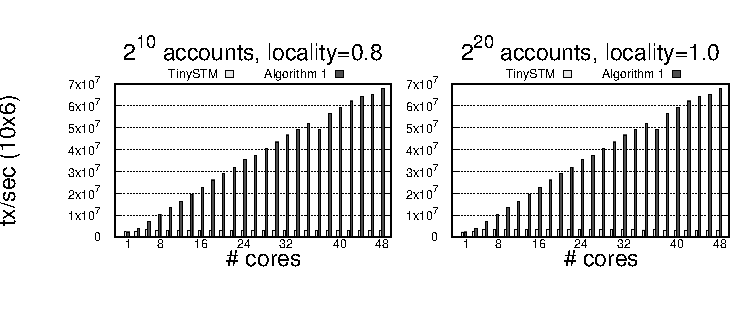
\includegraphics[scale = 1.0]{results/intset/bank.pdf}
	\caption{Bank Benchmark. Left: 80\% locality. Right: 100\% locality.\label{fig:benchmarking:bank}}
\end{figure}

\begin{figure}[!t]
	\centering
	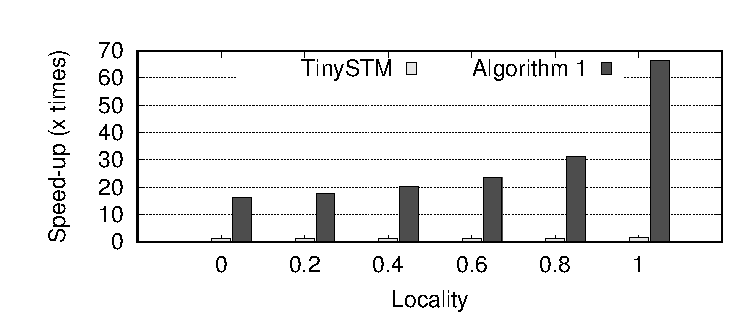
\includegraphics[scale = 0.8]{results/bank-speedup/bank-speedup.pdf}
	\caption{Bank Benchmark. Speed-up of our algorithm for different locality levels. In this experiment, we always use 48 cores.\label{fig:benchmarking:bank:speedup}}
\end{figure}


\subsection{Benchmark: Linked-list}

The linked-list benchmark consists in modifying a sorted linked list concurrently. 
Each thread randomly adds or removes a node from the list. 
We run this benchmark with a range of 512 (meaning that each thread randomly adds/removes a value comprised between -255 and +256) and a linked list initialized with 256 values.
Figure~\ref{fig:benchmarking:llrb}(left) reports our results.

The results show that the global clock outperforms our implementation. 
This is due to the high contention in this application that causes our optimistic algorithm to abort \ft{that's not the right verb} many transactions.

\begin{figure}[!t]
	\centering
	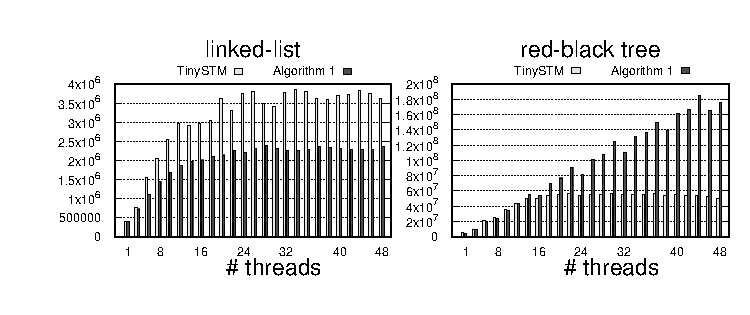
\includegraphics[scale = 1.0]{results/intset/ll-rb.pdf}
	\caption{Linked-list (left) and Red-Black tree (right) benchmarks. Y-axis: transactions/sec. \label{fig:benchmarking:llrb}}
\end{figure}

\subsection{Reb-black tree}

The red-black tree benchmark is similar to the linked-list benchmark except that the values are stored in a self-balancing binary search tree. 
We run this benchmark with a range of $10^7$ values, and a binary tree initialized with $10^5$ values.
Figure~\ref{fig:benchmarking:llrb}(right) reports our results.

When using the global clock, the performance of this application improves linearly up to 12 threads. 
It then stalls to approximately 50 millions transactions per second.

On this application, our implementation scales linearly as the number of threads grows. 
It achieves 176 millions transactions per second with 48 threads.
%
In this benchmark, the likelyhood of a concurrent transaction is very low because of the high number of values in the tree. However,\ft{explain why the global clock performs poorly}.
%

\section{Related Work}
\labsection{relatedwork}

Software transactional memory systems must handle a tradeoff between consistency and performance.
It is however impractical to take into account all possible combinations of read and write conflicts, as it would lead to leargely inefficient solutions. 
%A conflict detection, taking into account all possible combinations of read and write conflicts would just not be efficient. 
Therefore, several mechanisms were introduced to reduce the effort of conflict detection and increase concurrency. 
DSTM~\cite{herlihy2003software} validates all previously accessed object when a new object is about to be opened. 
However, this approach does not scale, and its complexity is quadratic to the number of opened objects within a transaction.

Several time-based STM designs use a global version clock (e.g., Riegel \cite{riegel2006lazy}) to avoid the effort of incrementally validating the read set at commit time. 
TinySTM~\cite{FelberFMR10} is a time-based STM that uses a lazy snapshot technique. 
On commit the TM assigns a timestamp from the global clock to the currently written objects. 
Any transaction constructs a snapshot of linearization points for ensuring consistency. 
By keeping a validity interval of timestamps, it can be verified whether a validation is really necessary. 
We use TinySTM as baseline for our evaluation.

The authors of \cite{zhang2008commit} compare Transactional Locking II (TL2)~\cite{dice2006transactional}, Lazy Snapshot (LSS)\cite{riegel2006lazy} and Global Commit Counter (GCC)~\cite{spear2006conflict}. 
All of them require a new timestamp for each update transaction (total order).
Their approach perform unnecessary updates on the global counter thus leading to unnecessary validations. 
The authors provide several commit alternatives to solve these issues and reducing further unnecessary validations.

New challenges arise when considering multicore architectures and cache coherency strategies for NUMA architectures. 
Clock contention~\cite{6121290} is one of the major issues. 
In a multi-core system with several processors and separate caches, cache coherence messages are required on each update of the clock, which happens frequently. 
Transaction throughput is therefore limited.

To tackle these issues the authors of \cite{Avni:2008} introduce TL2C, which consider a distributed counter --- one per thread. 
The clock values propagate to a \emph{dlock} table with $n-1$ lock entries of different threads. 
During a validation phase, this cache is used, which may however lead to unnecessary aborts. 
Another issue is that the storage of the timestamps might not scale with the number of threads.

In \cite{6121290} the authors adapt TL2 to TrC-MC~\cite{chan2011trc} (transactional consistency for multicore), which groups threads into so-called \textit{zones}. 
Zones share a clock and a clock table.\vs{add a sentence to explain why this is relevant} 
To avoid unnecessary aborts, TrC-MC adopts a timestamp extension mechanism.
TrC-MC compares favourably against TL2 in terms of aborted transsactions.  
%Still the number of aborts are increased, while lower than caused by TL2C.

\vs{add ProteusTM~\cite{didona2016proteustm}}
\vs{add PODC'10 NUMA-aware TM ~\cite{Lu:2010:BAN:1835698.1835713}}
\vs{add ~\cite{Mohamedin:2016:DNC:2851141.2851189}}

\vs{Complete section with 2/3 sentences about how why NumaSTM is different }
\vs{cite ~\cite{nguyen2017scalable}}
%%Why is distributed TM not a relevant work
%%get some more from 612...
%%TODO, why is ours better?

% RWCounter (Lev & Moir) 
% this solution is still global 

% Maintaining Consistent Transactional States without a Global Clock, Avni & Shavit
% space suage: O(m) per thread.
% each transaction got a vector clock inddicating the ts at which other transactions started
% each location got a timestamp pair (x.ts,x.owner), where x.owner is the thread that wrote x last.
% upon reading x, T compare x.ts to  its ts and abort if x.ts[x.owner] > T.ts[x.owner]
% no forward reading possible, thus more false abprt:
%
% This algorithm is SSER but has two main disadvantages
% 1) 
% ``We argue that a TLC transaction will always fail if it attempts 
% to read a location that was written by some other transaction after it started.''
% example of spurious abort: w_p(x).c_p.r_q(x).w_q(y).c_p.r_{q'}(y).a_{q'}.r_{q'}(x).a_{q'}
% the progress property of this STM is very weak, namely
% if the transaction starts from a quescient state and it repeatdly executed and there is no concurrent transaction, then it commits.
% 2) abortion due to non-causally consistent snapshot
% our appraoch does not have this problem


%% With multiple CPUs, each with its own clock, its impossible to guarantee that the crystals
%% don’t differ after some amount of time even when initially set accurately. In practice, all clocks
%% counters will run at slightly different rates. This clock skew brings several problems that can occur
%% and several solutions as well, some more appropriate than others in certain contexts.
%% The Time Stamp Counter was once an excellent high-resolution, low-overhead way for a program to get CPU timing information. With the advent of multi-core/hyper-threaded CPUs, systems with multiple CPUs, and hibernating operating systems, the TSC cannot be relied upon to provide accurate results — unless great care is taken to correct the possible flaws: rate of tick and whether all cores (processors) have identical values in their time-keeping registers. There is no promise that the timestamp counters of multiple CPUs on a single motherboard will be synchronize
%% Relying on the TSC also reduces portability, as other processors may not have a similar feature

%% Thanks for all the inputs: Here's the conclusion for this discussion: The TSCs are synchronized at the initialization using a RESET that happens across the cores and processors in a multi processor/multi core system. And after that every Core is on their own. The TSCs are kept invariant with a Phase Locked Loop that would normalize the frequency variations and thus the clock variations within a given Core and that is how the TSC remain in sync across cores and processors.

%% https://stackoverflow.com/questions/10921210/cpu-tsc-fetch-operation-especially-in-multicore-multi-processor-environment
%% https://github.com/dterei/tsc

%% PCL theorem

% the alg. of shvit et al. exhibits a very weak progress property, namely if the transaction is retried infinitely often it eventually commits.

%%   Computer designs that exploit data locality with multiple cache levels, such as non-uniform memory architectures (NUMA), have to reduce the amount of global operations to improve application performance or take special care to address traffic congestions\cite{dashti2013traffic}.


\section{Conclusion}
\labsection{conclusion}

Transactional memory systems must handle a tradeoff between consistency and performance.
It is impractical to take into account all possible combinations of read and write conflicts, as it would lead to largely inefficient solutions.
%% For instance, accepting $\RCAD$ histories brings only a small performance benefits in the general case~\cite{hans16}.

%Inspired by line of research, 
This paper introduces a new consistency criterion, named stricter serializability ($\SPSER$).
Workloads executed under $\SPSER$ are opaque when the object graph forms a tree and transactions traverse it top-down.
We present an algorithm to attain this criterion together with a proof of its correctness.
Our evaluation based on a fully implemented prototype demonstrates that such an approach is very efficient in weakly-contended workloads.

% move from SSER to SSER+ (i.e., alg. transform) ?



{
  %\footnotesize
  \bibliographystyle{splncs04}
  \bibliography{bib/nicolas,bib/psutra,bib/mshapiro,bib/paper}
}

\clearpage
\appendix
\section{From strict serializability to opacity}
\labappendix{from}

\input{algorithms/from}

\begin{lemma}
  \lablem{from:0}
  Consider some history $h$ such that $(\committed{h},<_{\committed{h}})$ is acyclic.
  Every linearization $\lambda$ of $(h|\committed{h})$ according to $\closureOf{<_{\committed{h}}}$ is legal.  
\end{lemma}

\begin{proof}
  Let $\lambda$ be the sequential history equivalent to $(h|\committed{h})$ in which transactions are ordered according to $\closureOf{<_{\committed{h}}}$.
  %
  Choose some transaction $T_i$ in $\lambda$.
  For every read operation $r_i(x_j)$ in $h$, $T_j <_{\committed{h}} T_i$ holds.
  Hence $w_j(x_j)$ precedes $r_i(x_j)$ in $\lambda$.
  Then, by contradiction, consider some $T_k$ in $\committed{h}$ such that $T_j \hb_{\Lambda} T_k \hb_{\Lambda} T_i$ and $w_k(x_k)$ is in $h$.
  Since both $T_j$ and $T_k$ write $x$ and $T_j \hb_{\lambda} T_k$ holds, necessarily $x_j \ll_h x_k$ is true.
  Thus, $T_i <_{\lambda} T_k$ holds.
  Contradiction.
\end{proof}

\begin{lemma}
  \lablem{from:1}
  Consider some legal history $h$.
  Let $T_i$ and $T_j$ be two transactions in $h$ such that $h = h_1 T_i T_j h_2$, for some $h_1$ and $h_2$.
  If $\readSetOf{T_i} \inter \writeSetOf{T_j} = \emptySet$, $\readSetOf{T_j} \inter \writeSetOf{T_i} = \emptySet$ and $\writeSetOf{T_j} \inter \writeSetOf{T_i} = \emptySet$ are all true, then history $h' = h_1 T_j T_i h_2$ is legal and equivalent to $h$.
\end{lemma}

\begin{proof}
  Clearly $h'$ is equivalent to $h$.
  Then, consider some read operation $r_l(x_k)$ in $h'$.
  As $h$ is legal, $T_k$ is the last transaction writing to $x$ before $T_l$ in $h$.
  We now prove that this is still the case in $h'$.  
  If $r_l(x_k)$ occurs in $h_1$, the result is obvious.
  Otherwise, if $T_l = T_i$, this property is also true since $\readSetOf{T_i} \inter \writeSetOf{T_j} = \emptySet$.
  A symmetrical argument holds for the case $T_l = T_j$.
  Last, in case $T_l$ occurs in $h_2$, $\writeSetOf{T_j} \inter \writeSetOf{T_i} = \emptySet$ implies the result.
\end{proof}

\begin{proposition}
  \labprop{from:2}
  Consider a history $h$ such that $\RSG(\committed{h},\ll_{\committed{h}})$ is acyclic for some version order $\ll_h$.
  History $h$ is opaque ($h \in \OPA$) if the transactions aborted in $h$ observe strictly consistent snapshots for $\ll_h$.
\end{proposition}

\begin{proof}
  
  Since history $h$ is in $\SSER$, \reflem{from:0} tells us that we can linearize $(h|\committed{h})$ following relation $\closureOf{<_{\committed{h}}}$.
  Let $\lambda$ be such a history.

  \refalg{from} takes as input $\lambda$, copy it to variable $\Lambda$, then add appropriately to $\Lambda$ the transactions aborted in $h$ to form a legal history equivalent to $h$.
  When adding an aborted transaction (\refline{from:2}), \refalg{from} permutes some of its dependencies in $\Lambda$ (\reflines{from:3}{from:5}) to maintain the legality of $\Lambda$ at each step of the rewriting.

  Below, we prove that when \refalg{from} outputs history $\Lambda$, this history is both legal and equivalent to $h$.
  To this end, let us first observe that the following invariants are true in \refalg{from}.  
  \begin{itemize}

  \item $\tlGlobally(<_{\committed{h}} \subseteq \hb_{\Lambda})$.
    By induction.
    From the pseudo-code at \refline{from:1}, this is initially true.
    %
    Consider two transactions $T_k$ and $T_l$ with $T_k <_{\committed{h}} T_l$.
    Since $<_{\committed{h}} \subseteq <_h$, $T_k$ and $T_l$ are not permuted at \refline{from:5}.
    Because an aborted transaction is added to $\Lambda$ at \refline{from:8}, the invariant still holds after executing this line.
    Hence, the main loop (\reflines{from:2}{from:8}) maintains the invariant.

  \item $\tlGlobally(\Lambda\text{ is legal})$.
    By induction.
    Initially, this is true (\refline{from:1}).
    %
    Consider transactions $T_k$ and $T_l$ as defined at \reflinestwo{from:3}{from:4}.
    Since $\neg (T_k <_h T_l)$ and $\Lambda$ is sequential, $\writeSetOf{T_k} \inter \readSetOf{T_l} = \emptySet$, $\writeSetOf{T_k} \inter \readSetOf{T_l} = \emptySet$ and $\writeSetOf{T_k} \inter \writeSetOf{T_l} = \emptySet$ are all true.
    From \reflem{from:1}, $\Lambda$ is legal after applying \refline{from:5}.
    %
    Then, choose some transaction $T_i$ in $\Lambda$.
    If $T_i$ is committed in $h$, \refline{from:8} does not change the legality of $T_i$ as the transaction added to $\Lambda$ at that line is aborted.
    Assume now that $T_i$ is aborted.
    For some read $r_i(x_j)$, relation $T_j <_h T_i$ holds and $T_j$ is committed in $h$.
    Hence, after \refline{from:8}, $T_j$ precedes $T_i$ in $\Lambda$.
    Then, for the sake of contradiction, consider some $T_k$ such that $T_k \in \committed{h}$, $w_k(x_k) \in h$ and $T_j \hb_{\Lambda} T_k \hb_{\Lambda} T_i$.
    From $T_j \hb_{\Lambda} T_k$ and $<_{\committed{h}} \subseteq \hb_{\Lambda}$, we deduce that $x_j \ll_h x_k$ is true, leading to $T_i <_h T_k$.
    Then, since $T_k \hb_{\Lambda} T_i$ holds, $T_k \hb_h \Lambda[k] <_h T_i$ is true, with transaction $\Lambda[k]$ defined at \refline{from:6}.
    Hence, from the pseudo-code at \reflinestwo{from:4}{from:5}, we deduce by a short induction that $T_k <_h T_i$ also holds.
    This contradicts that the transitive closure of $<_h$ starting from $\{T_i\}$ is acyclic.    
  \end{itemize}
  Name $\Lambda'$ the output of \refalg{from}.
  From what precedes $\Lambda'$ is legal.
  In addition,
  \begin{itemize}
  \item $(\Lambda' \equiv h)$.
    Initially, history $\Lambda$ is equivalent to $\committed{h}$.
    Then, for every transaction $T_i$ aborted in $h$, after applying \refline{from:8} for $T_i$, $(\Lambda|T_i) = (h|T_i)$ holds.
    As a consequence, after \refline{from:9}, $\Lambda$ is equivalent to $h$.
  \item $(\hb_h \subseteq \hb_{\Lambda'})$.
    Consider that $T_i \hb_h T_j$ holds.
    %
    Below, we prove that when $T_i$ and $T_j$ are first added to $\Lambda$, $T_i \hb_{\Lambda} T_j$ is true.    
    Since $T_i <_h T_j$ holds, this order is maintained after each iteration at \refline{from:5}, leading to the result.
    %
    There are three cases to consider.
    \begin{inparaenum}
    \item[($T_i, T_j \in \committed{h}$.)]
      This case follows immediately from invariant $\tlGlobally(<_{\committed{h}} \subseteq \hb_{\Lambda})$.
    \item[($T_j$ is aborted.)]
      Transaction $T_j$ is inserted after $T_i$ at \refline{from:9}.
    \item[($T_i$ is aborted.)]
      By contradiction, consider that after inserting $T_i$ at \refline{from:9}, $T_j \hb_{\Lambda} T_i$ is true.
      We must have $T_j \hb_{\Lambda} \Lambda[k] <_h T_i$, with $\Lambda[k]$ defined at \refline{from:6}.
      Hence, from the pseudo-code at \reflinestwo{from:4}{from:5}, $T_j <_h T_i$ holds and $T_i$ does not observe a strictly consistent snapshot in history $h$.
    \end{inparaenum}
  \end{itemize}

  History $\Lambda$ is sequential, legal and preserves the real-time ordering in $h$.
  It follows that $h$ is opaque.  
\end{proof}



\end{document}
